\section{Debian}
\subsection{Attribution des paramètres réseaux}

Sur VirtualBox, sélectionner la machine virtuelle "Debian DM4", et cliquer sur \textit{Configuration} :
  \begin{figure}[h!]
     \begin{center}
         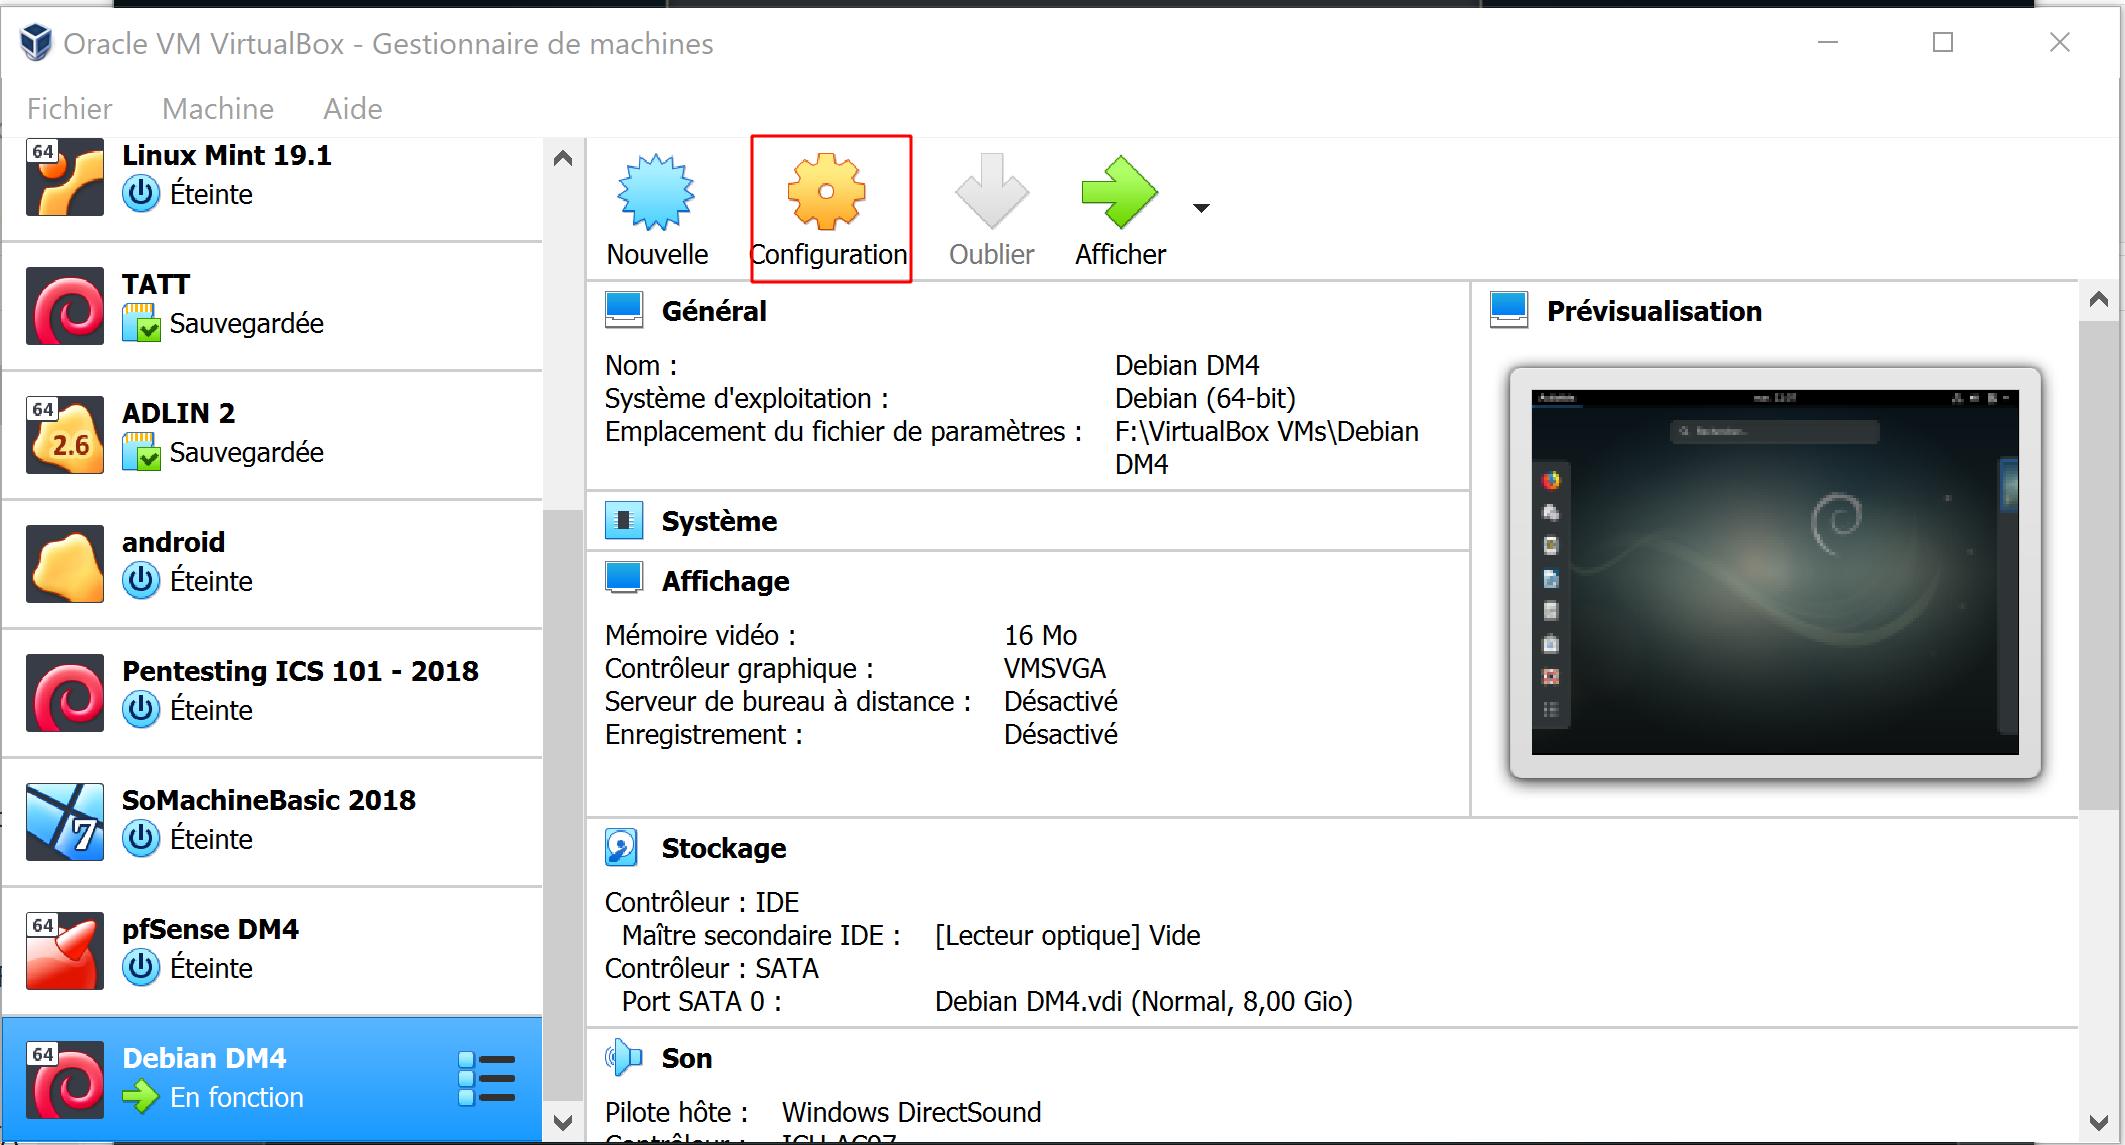
\includegraphics[scale=0.5]{Debian_screenshots/Config/1.png}
         \caption{Accès à la fenêtre de configuration de la machine virtuelle Debian}
         \label{Debian_screenshots/Config/1}
     \end{center}
  \end{figure}
  \FloatBarrier
     
Accéder à la section \textbf{Réseau}, puis dans l'onglet "Interface 1", sélectionner \textit{Réseau interne} comme mode d'accès réseau, avec "pfsense" comme nom :
  \begin{figure}[h!]
     \begin{center}
         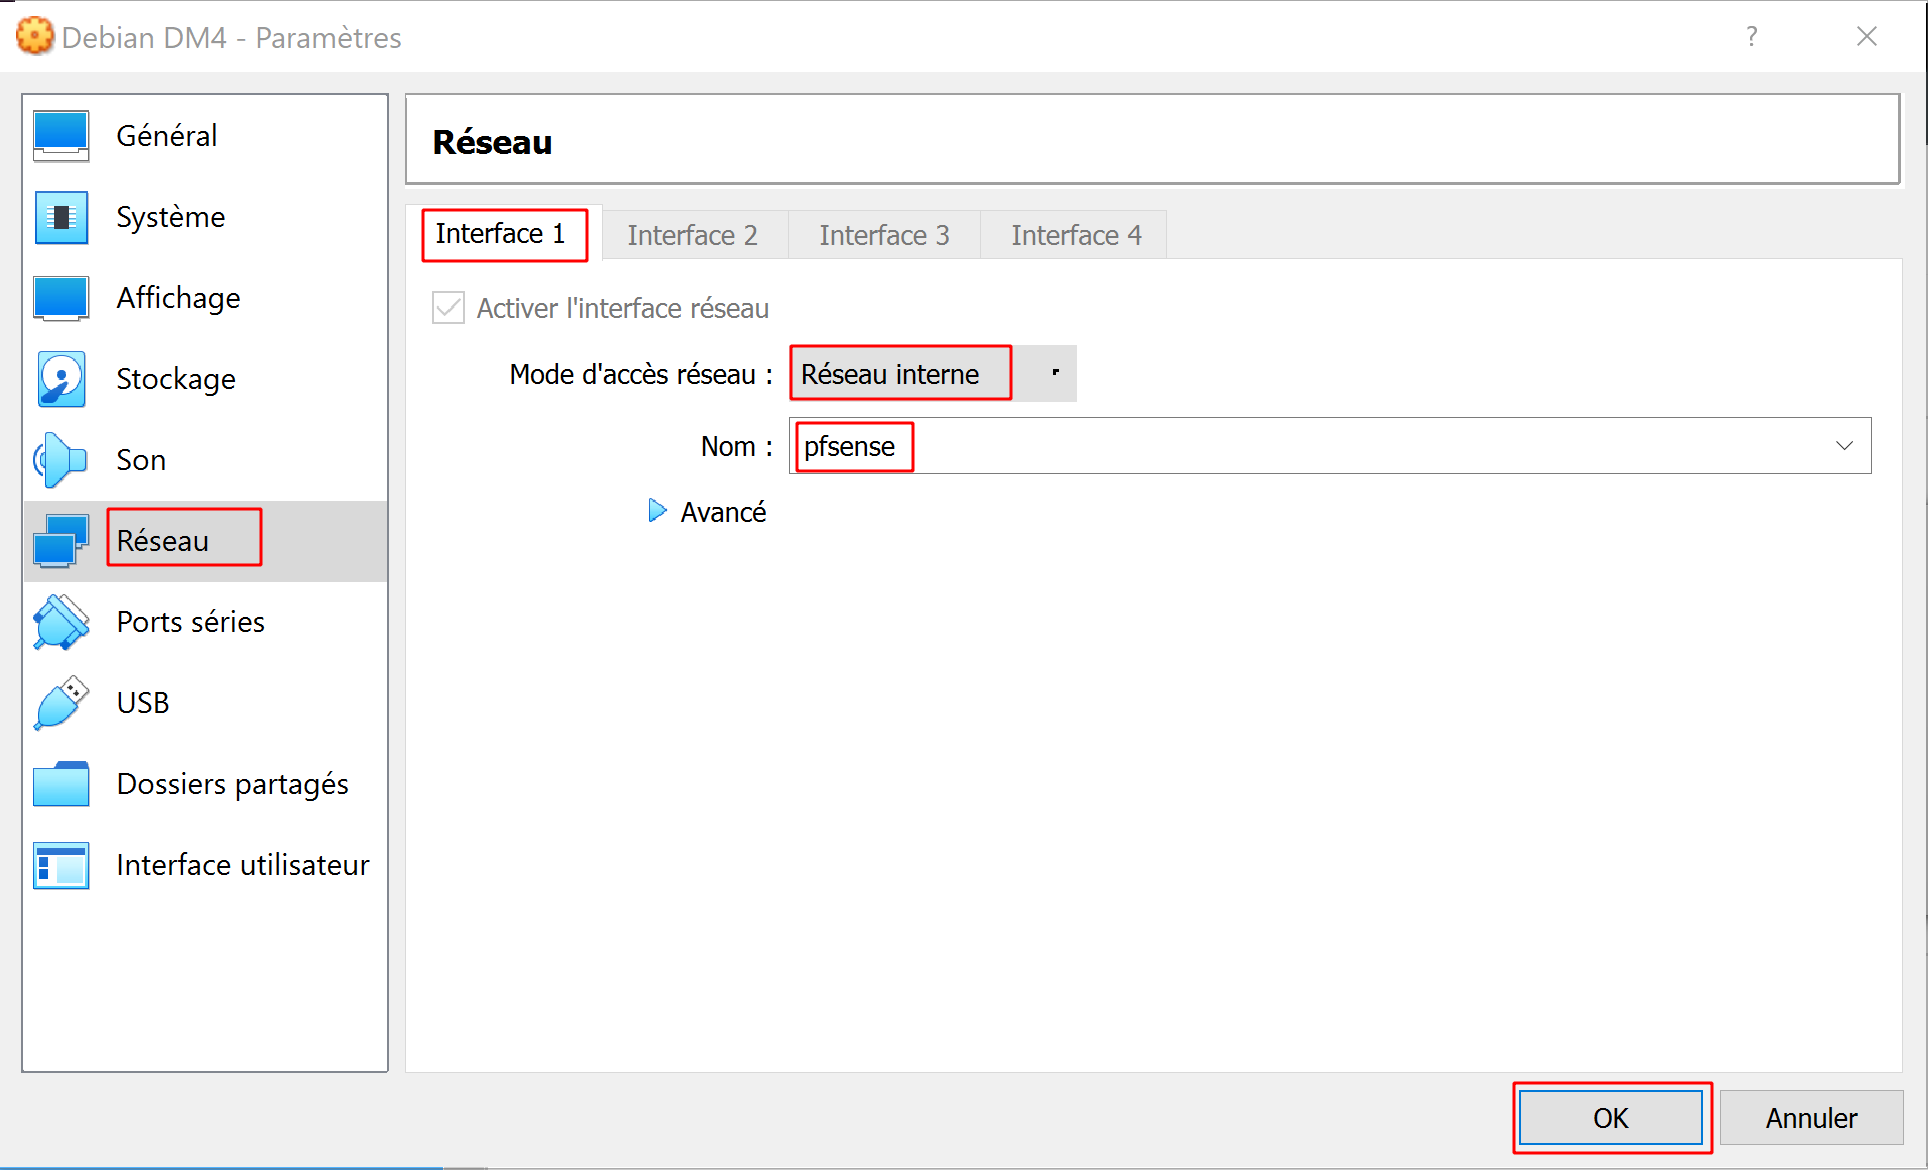
\includegraphics[scale=0.6]{Debian_screenshots/Config/2.png}
         \caption{Configuration réseau de la machine virtuelle Debian}
         \label{Debian_screenshots/Config/2}
     \end{center}
  \end{figure}
  \FloatBarrier

\pagebreak
Se connecter sur la machine virtuelle. Cliquer sur l'icône pour les réseaux, cliquer sur \textit{Connexion de Filaire en ...}, puis sur \textit{Paramètres filaires} :
  \begin{figure}[h!]
     \begin{center}
         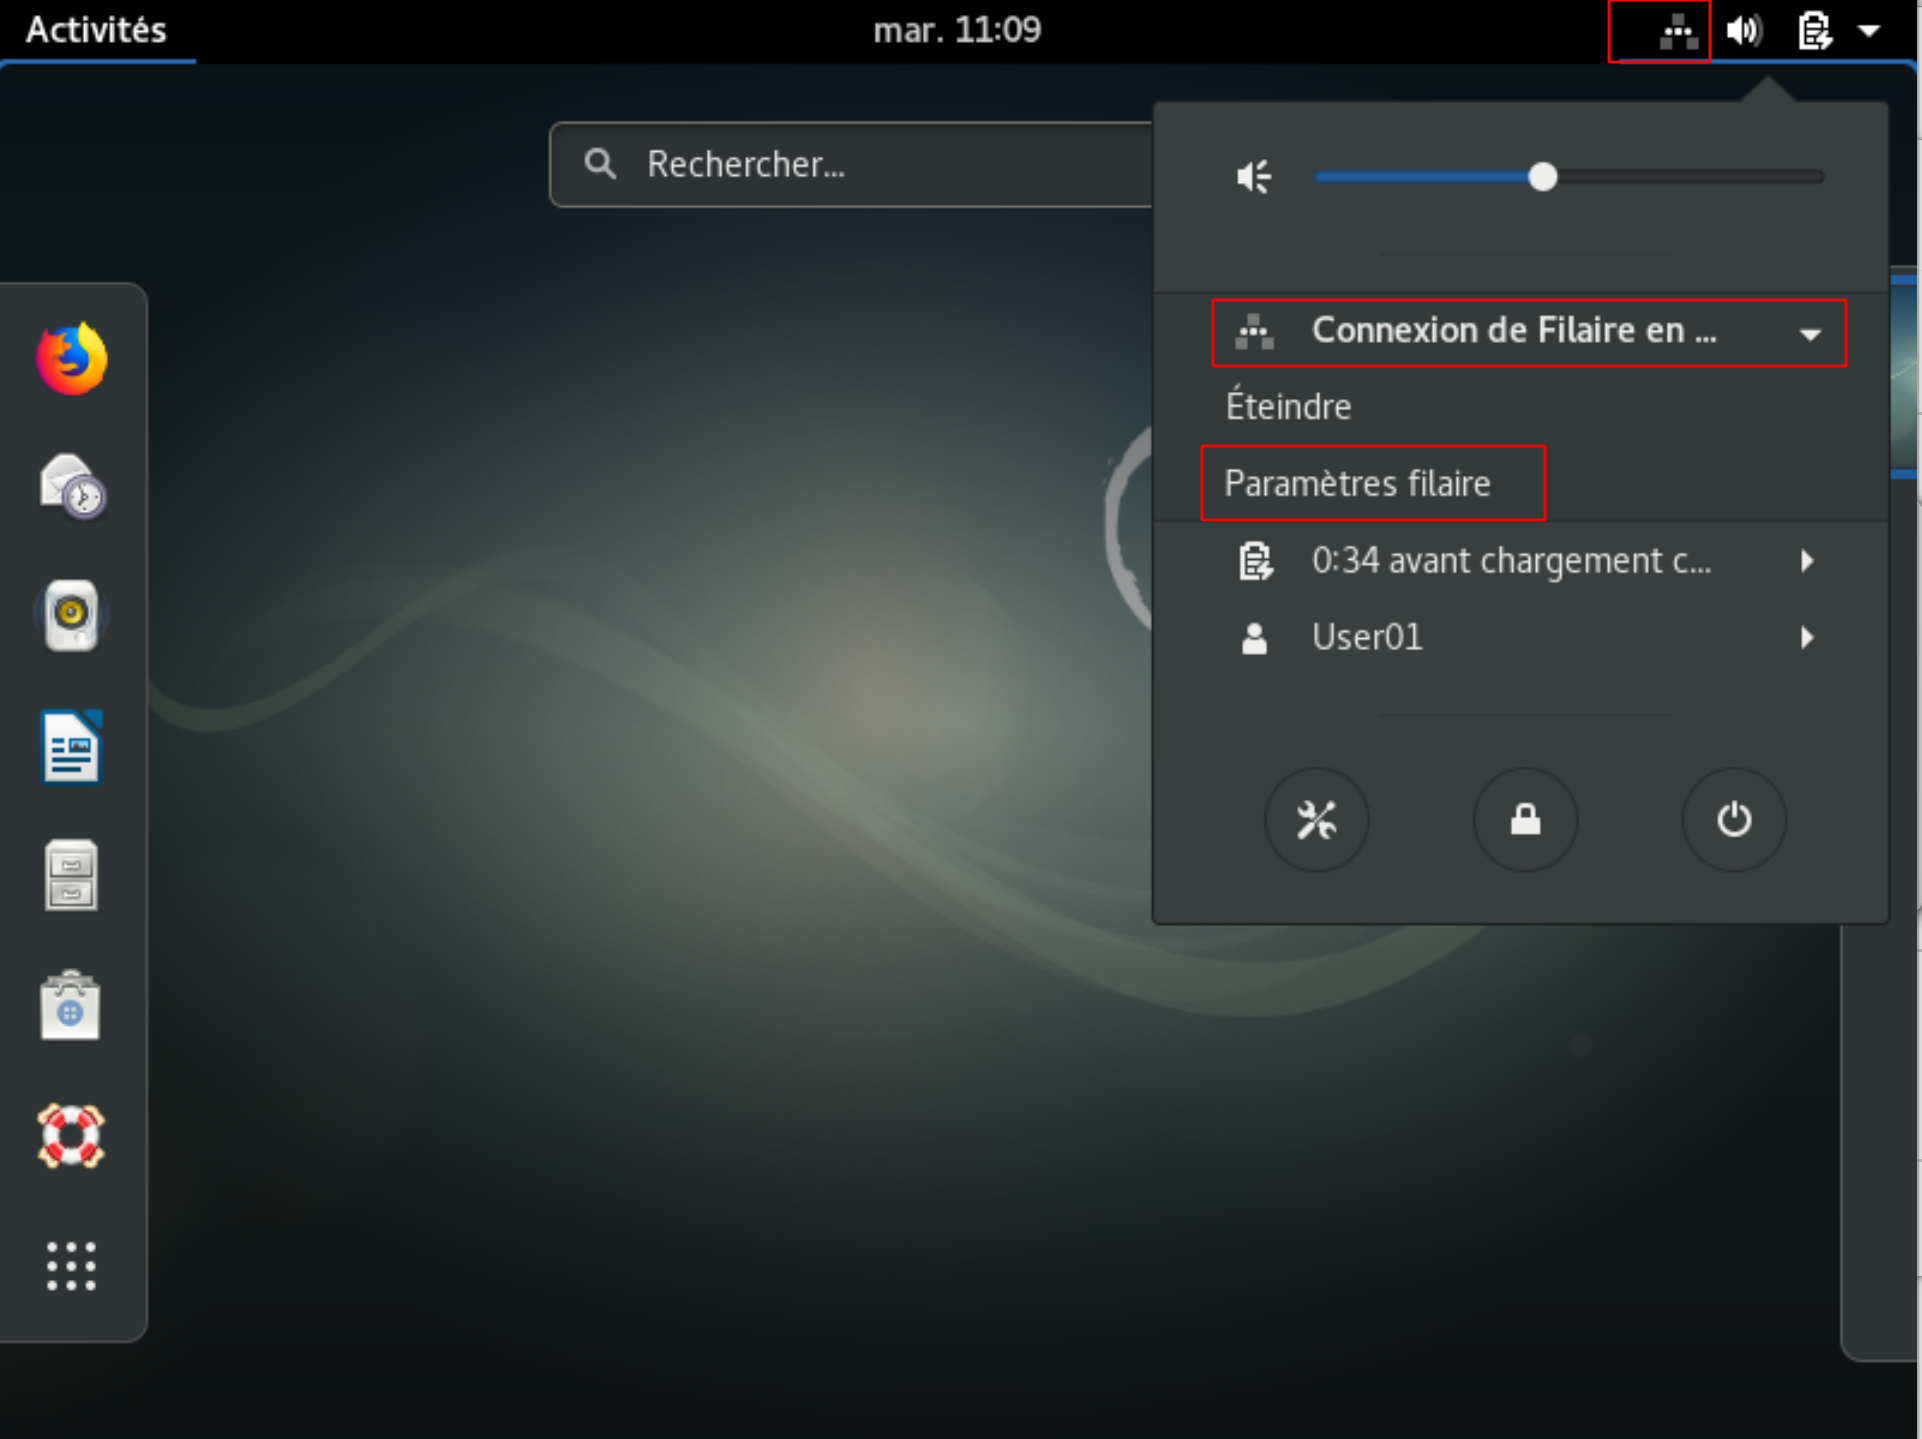
\includegraphics[scale=0.5]{Debian_screenshots/Config/3.png}
         \caption{Accès aux paramètres de configuration de connexion}
         \label{Debian_screenshots/Config/3}
     \end{center}
  \end{figure}
  \FloatBarrier
     
Sélectionner \textit{Filaire}, puis cliquer sur le bouton des paramètres :
  \begin{figure}[h!]
     \begin{center}
         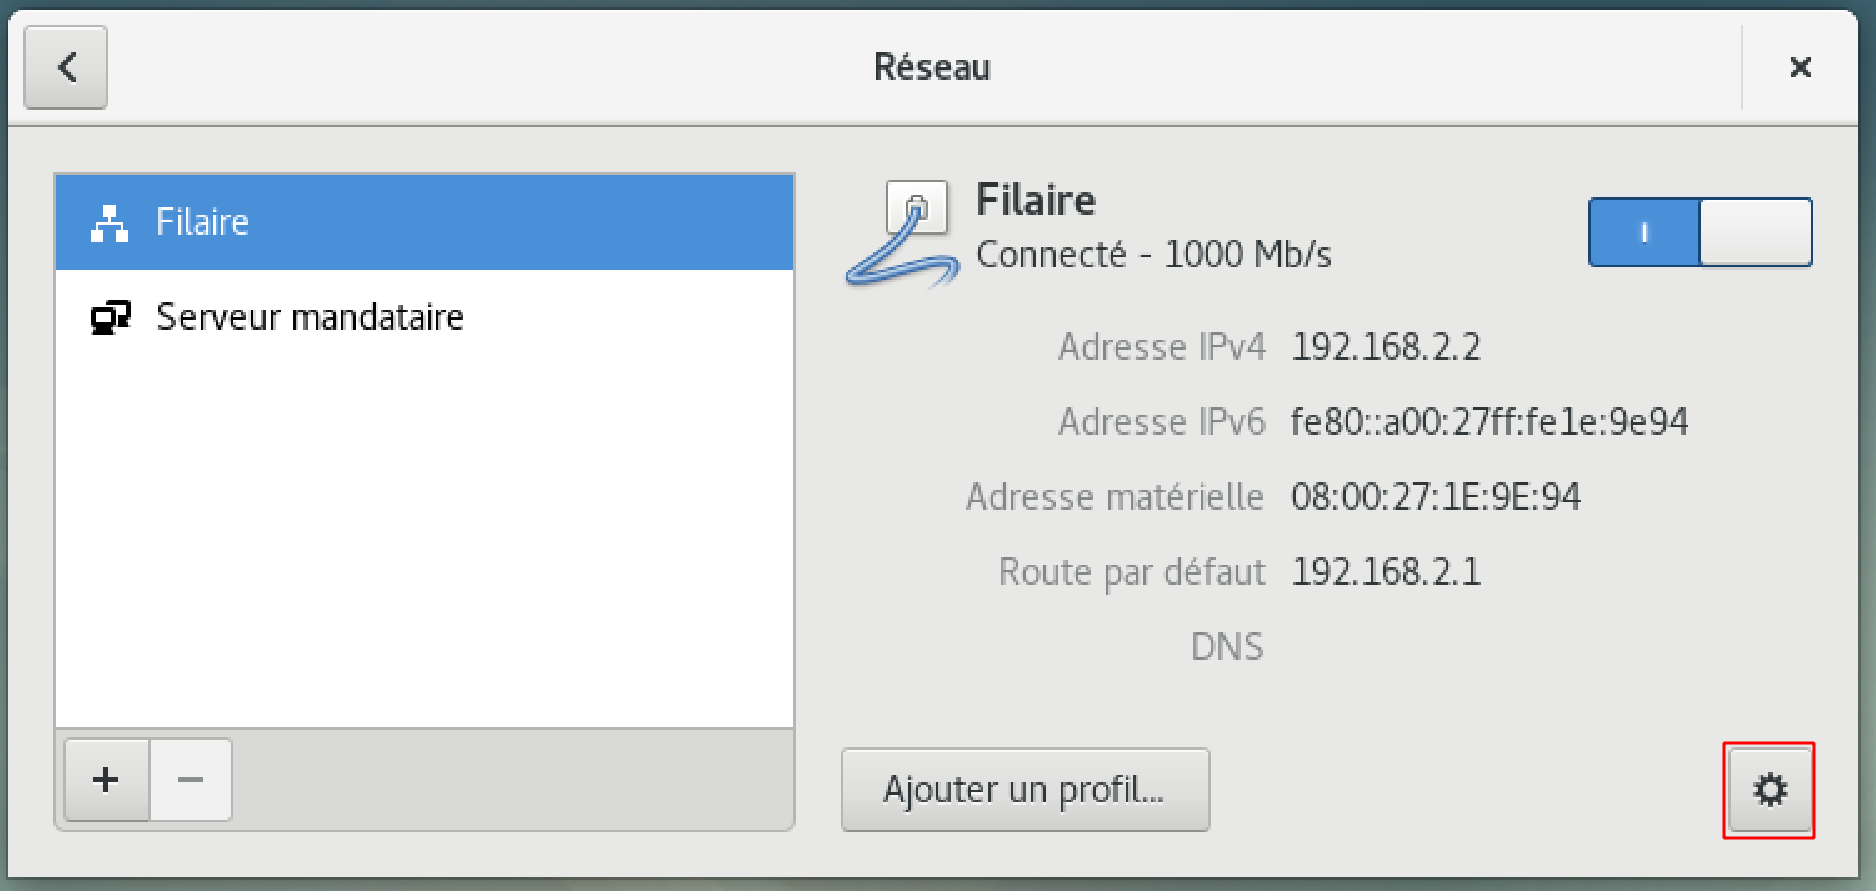
\includegraphics[scale=0.5]{Debian_screenshots/Config/4.png}
         \caption{Accès aux paramètres de connexion filaire}
         \label{Debian_screenshots/Config/4}
     \end{center}
  \end{figure}
  \FloatBarrier

\pagebreak
Aller dans la section \textit{IPv4}, puis sélectionner \textit{Manuel} afin de configurer les adresses suivantes : 192.168.2.2, 255.255.255.0 et 192.168.2.1. Cliquer sur \textit{Appliquer} :
  \begin{figure}[h!]
     \begin{center}
         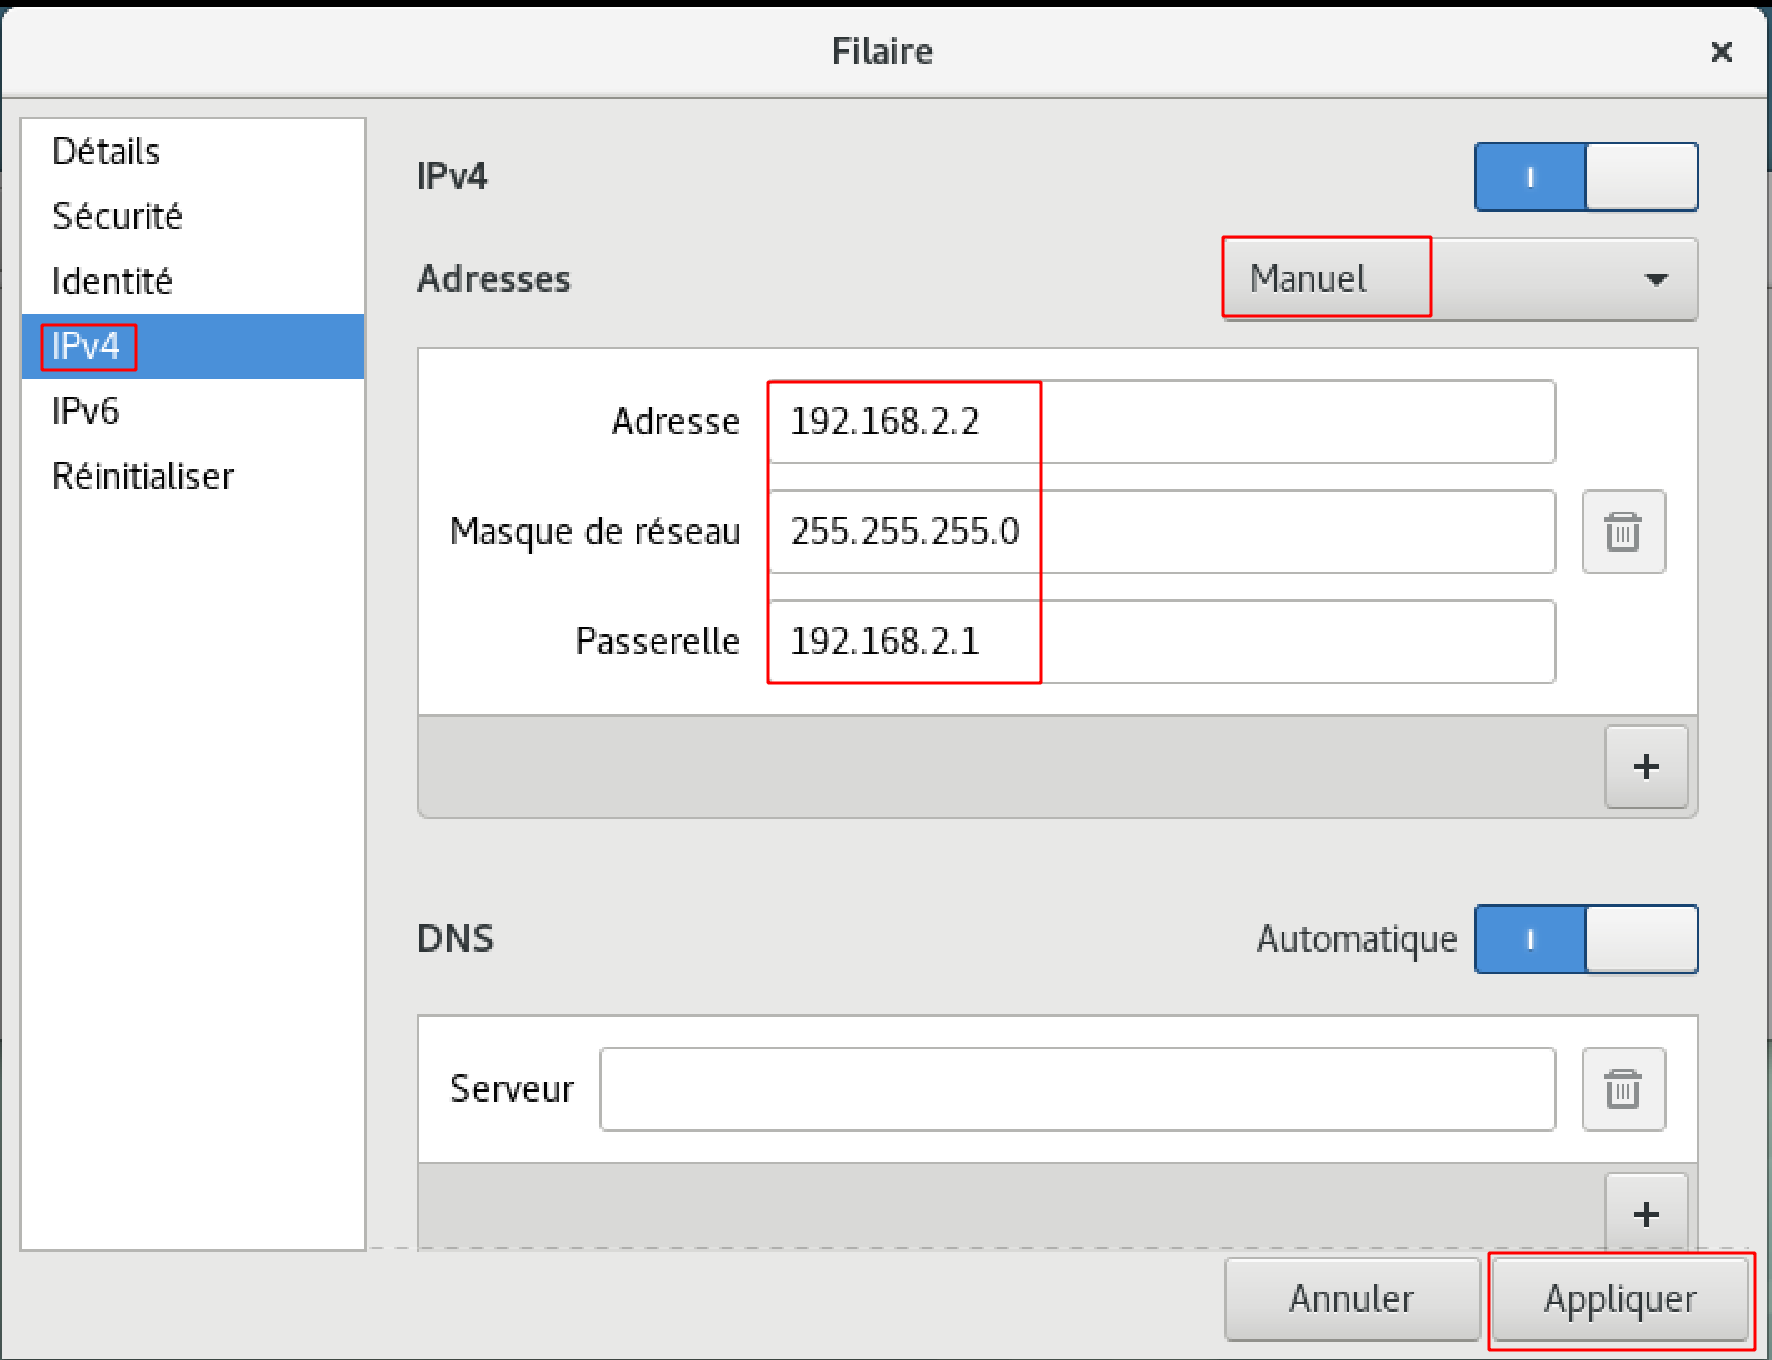
\includegraphics[scale=0.5]{Debian_screenshots/Config/5.png}
         \caption{Configuration des paramètres de connexion filaire en IPv4}
         \label{Debian_screenshots/Config/5}
     \end{center}
  \end{figure}
  \FloatBarrier
     
Ouvrir un navigateur, et se rendre à l'adresse "https://192.168.2.1" :
  \begin{figure}[h!]
     \begin{center}
         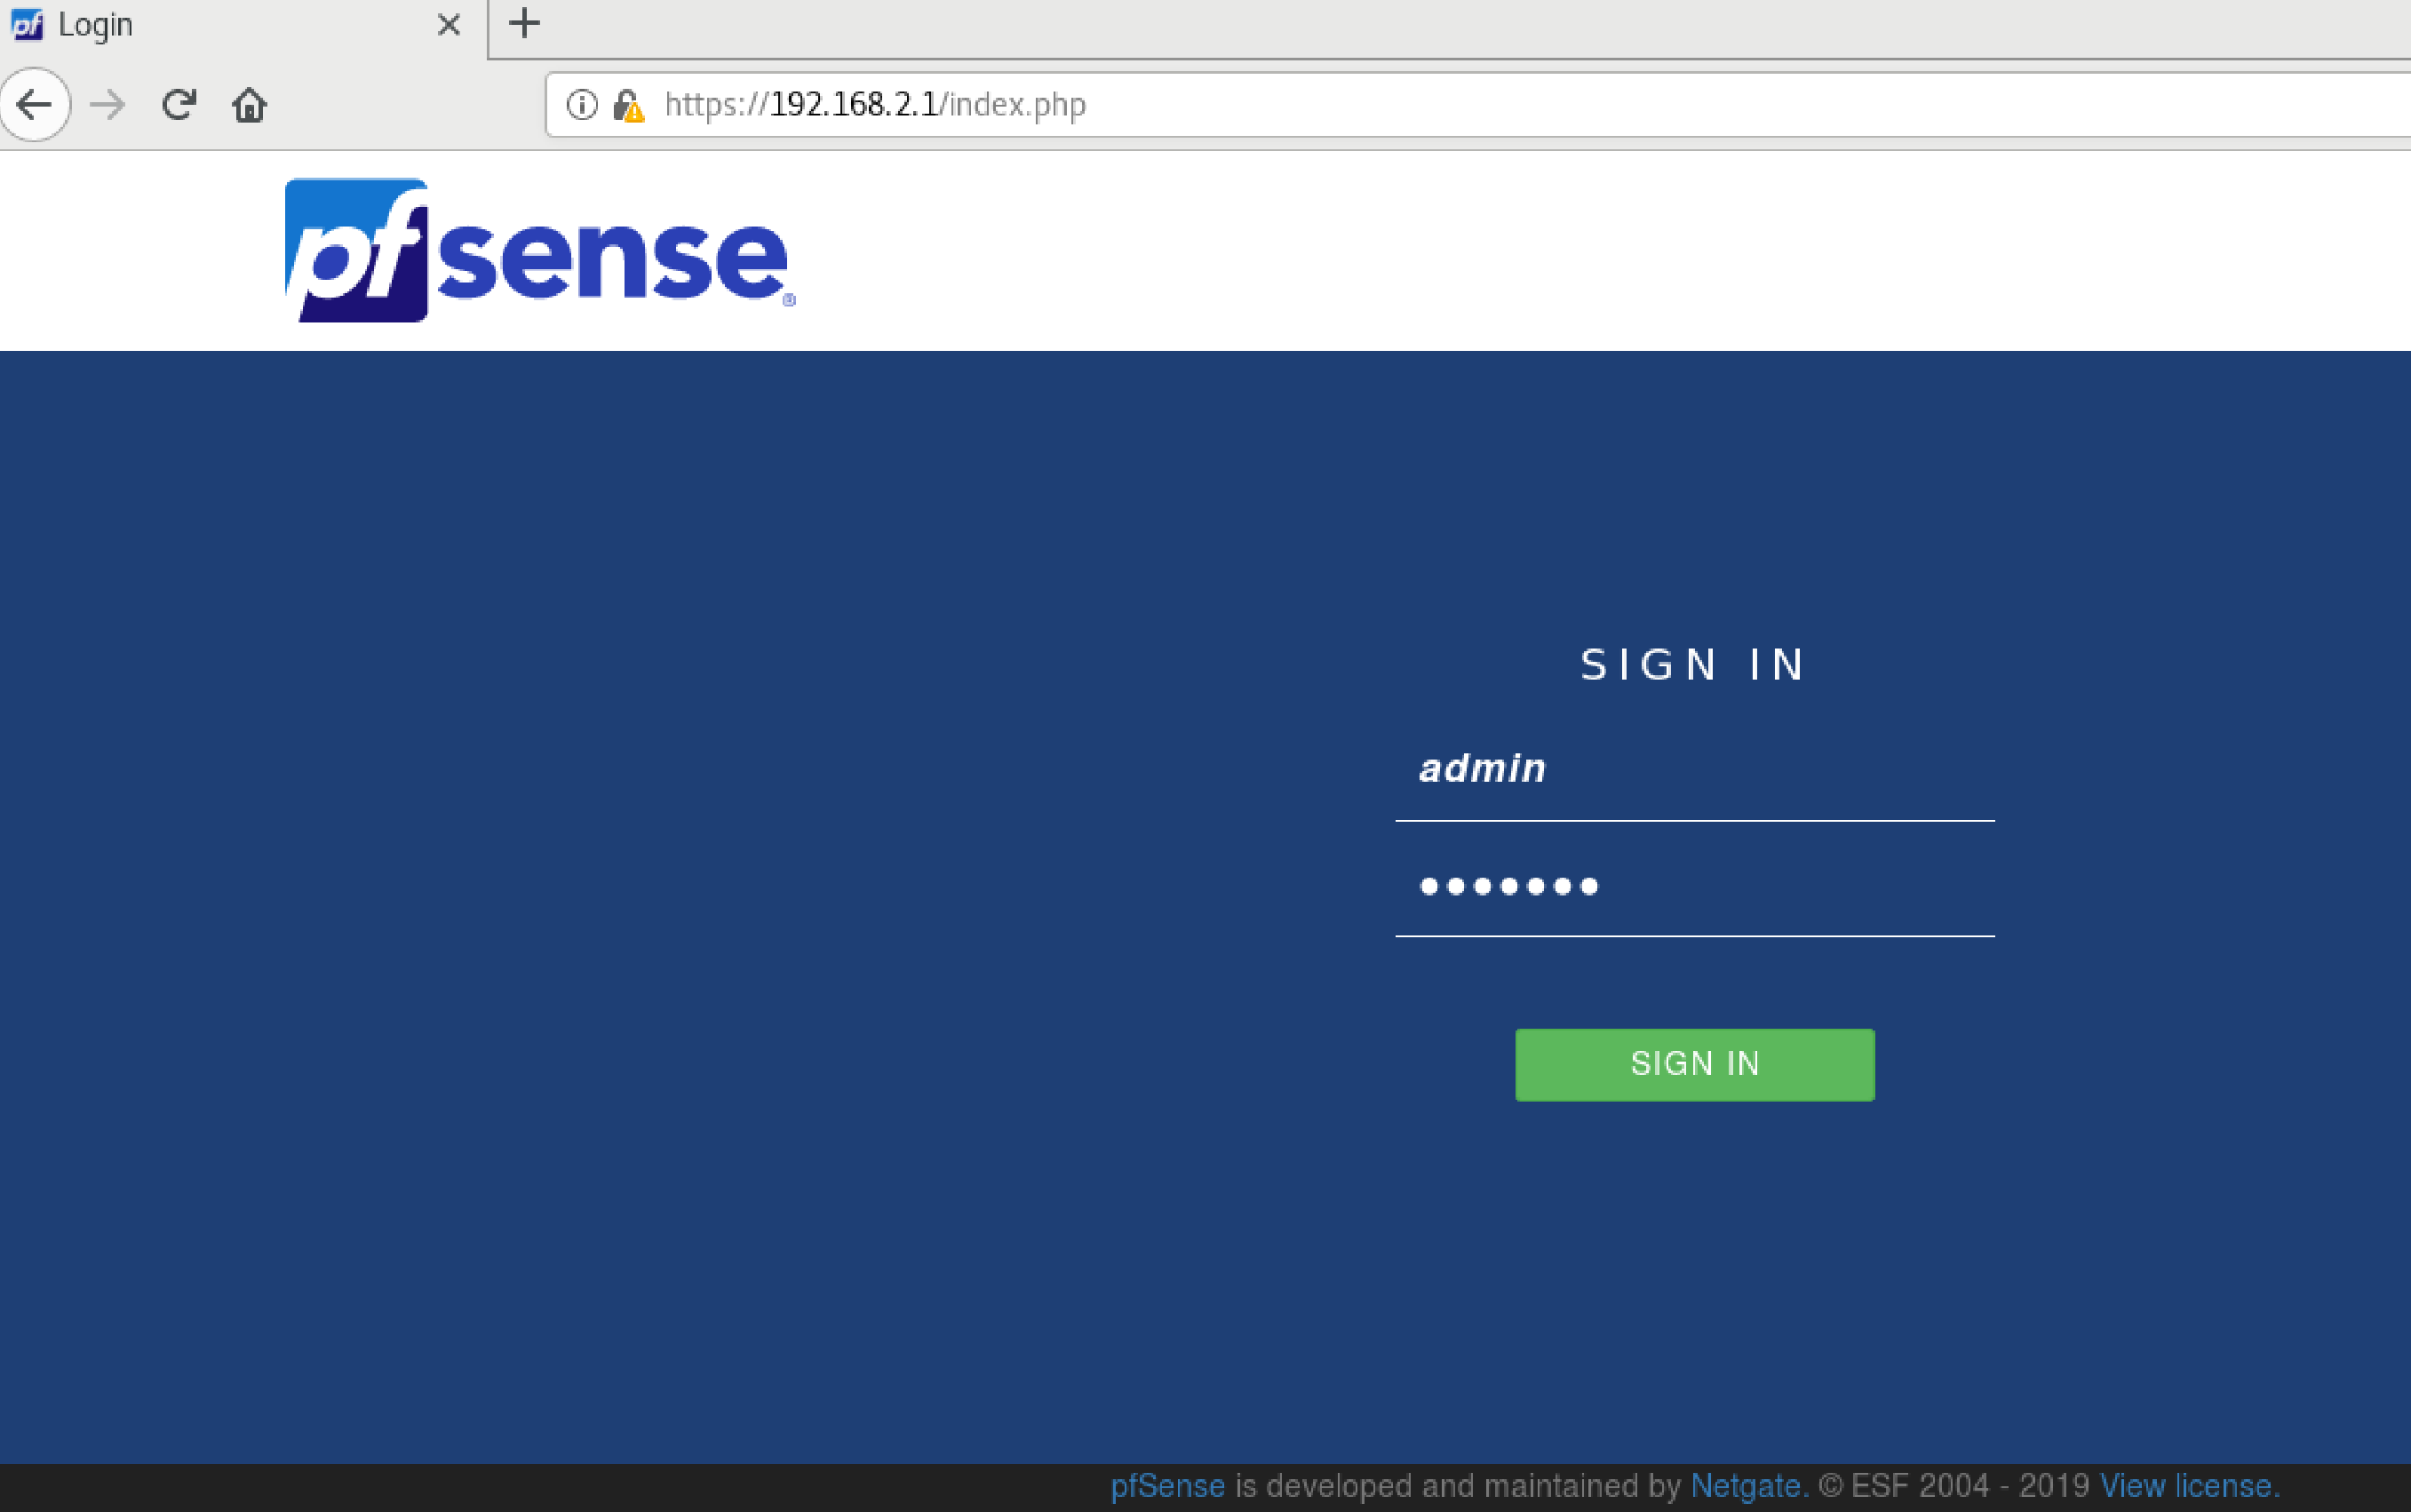
\includegraphics[scale=0.4]{Debian_screenshots/Config/6.png}
         \caption{Accès à la page web de configuration de pfsense}
         \label{Debian_screenshots/Config/6}
     \end{center}
  \end{figure}
  \FloatBarrier

\pagebreak
Ouvrir la fenêtre de configuration de la machine virtuelle de \textbf{pfsense}, et aller dans la section \textit{Réseau}. Se rendre dans l'onglet "Interface 3", cocher "\textit{Activer l'interface réseau}", sélectionner \textit{Réseau interne} comme mode d'accès réseau, avec pour nom "dmz". Cliquer sur \textit{OK} :
  \begin{figure}[h!]
     \begin{center}
         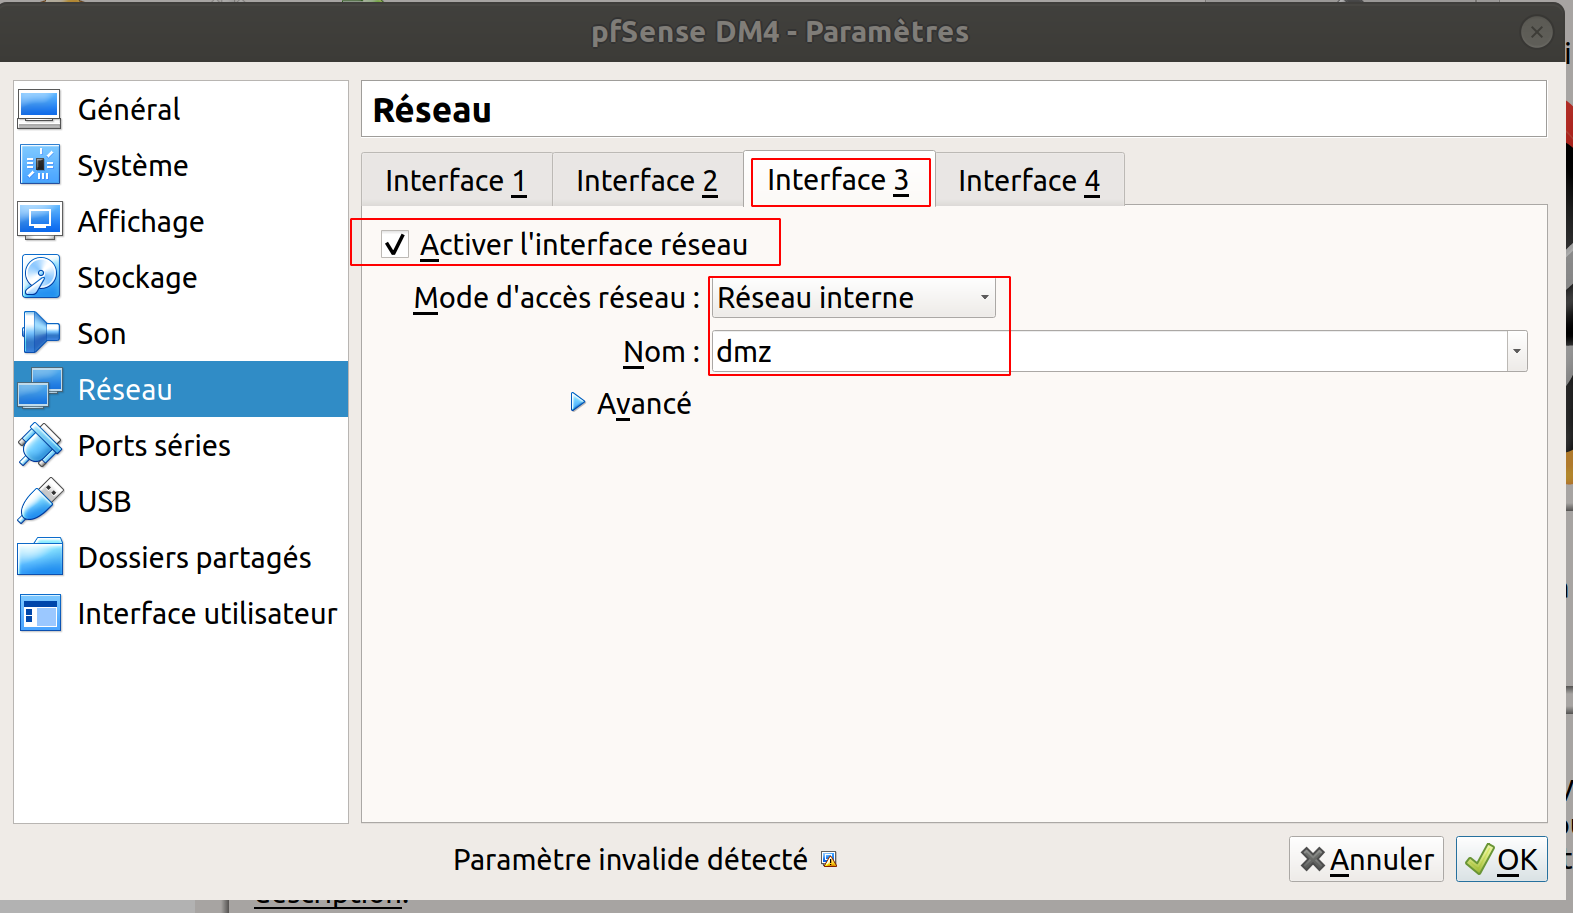
\includegraphics[scale=0.5]{Debian_screenshots/Config/7.png}
         \caption{Création d'un second réseau interne sur pfsense}
         \label{Debian_screenshots/Config/7}
     \end{center}
  \end{figure}
  \FloatBarrier
     
Sur la page web de configuration de pfsense, cliquer sur \textit{Interfaces} puis \textit{Assignments} :
  \begin{figure}[h!]
     \begin{center}
         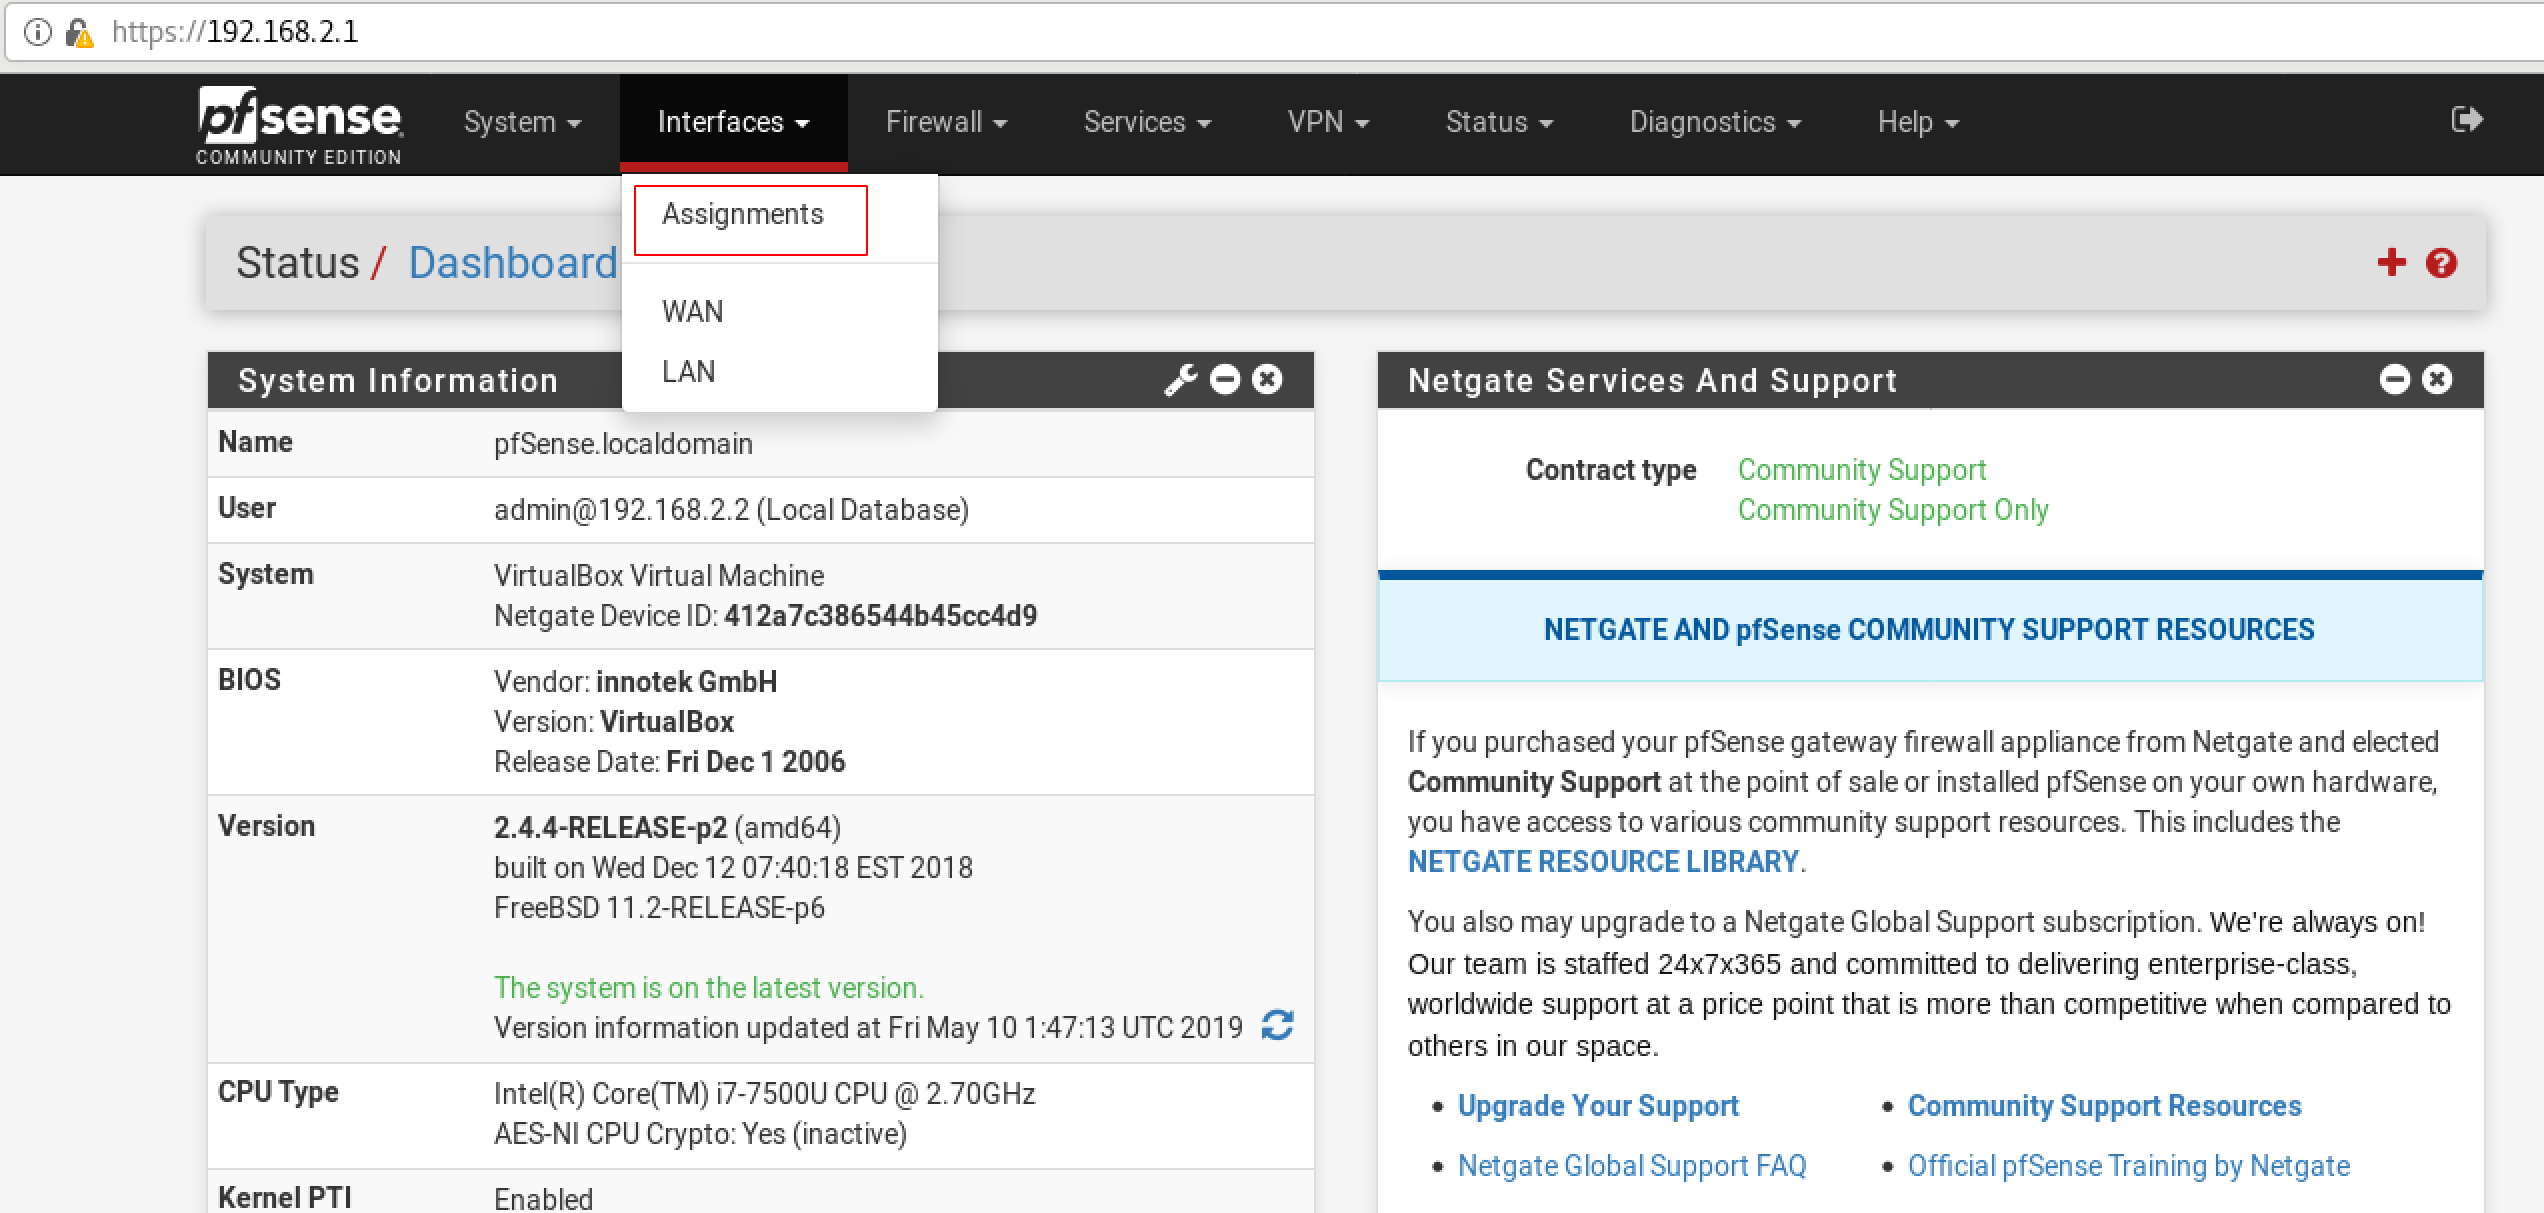
\includegraphics[scale=0.5]{Debian_screenshots/Config/8.png}
         \caption{Accès à l'assignation des interfaces sur la page web de configuration de pfsense}
         \label{Debian_screenshots/Config/8}
     \end{center}
  \end{figure}
  \FloatBarrier

\pagebreak
Cliquer sur le bouton \textit{Add} :
  \begin{figure}[h!]
     \begin{center}
         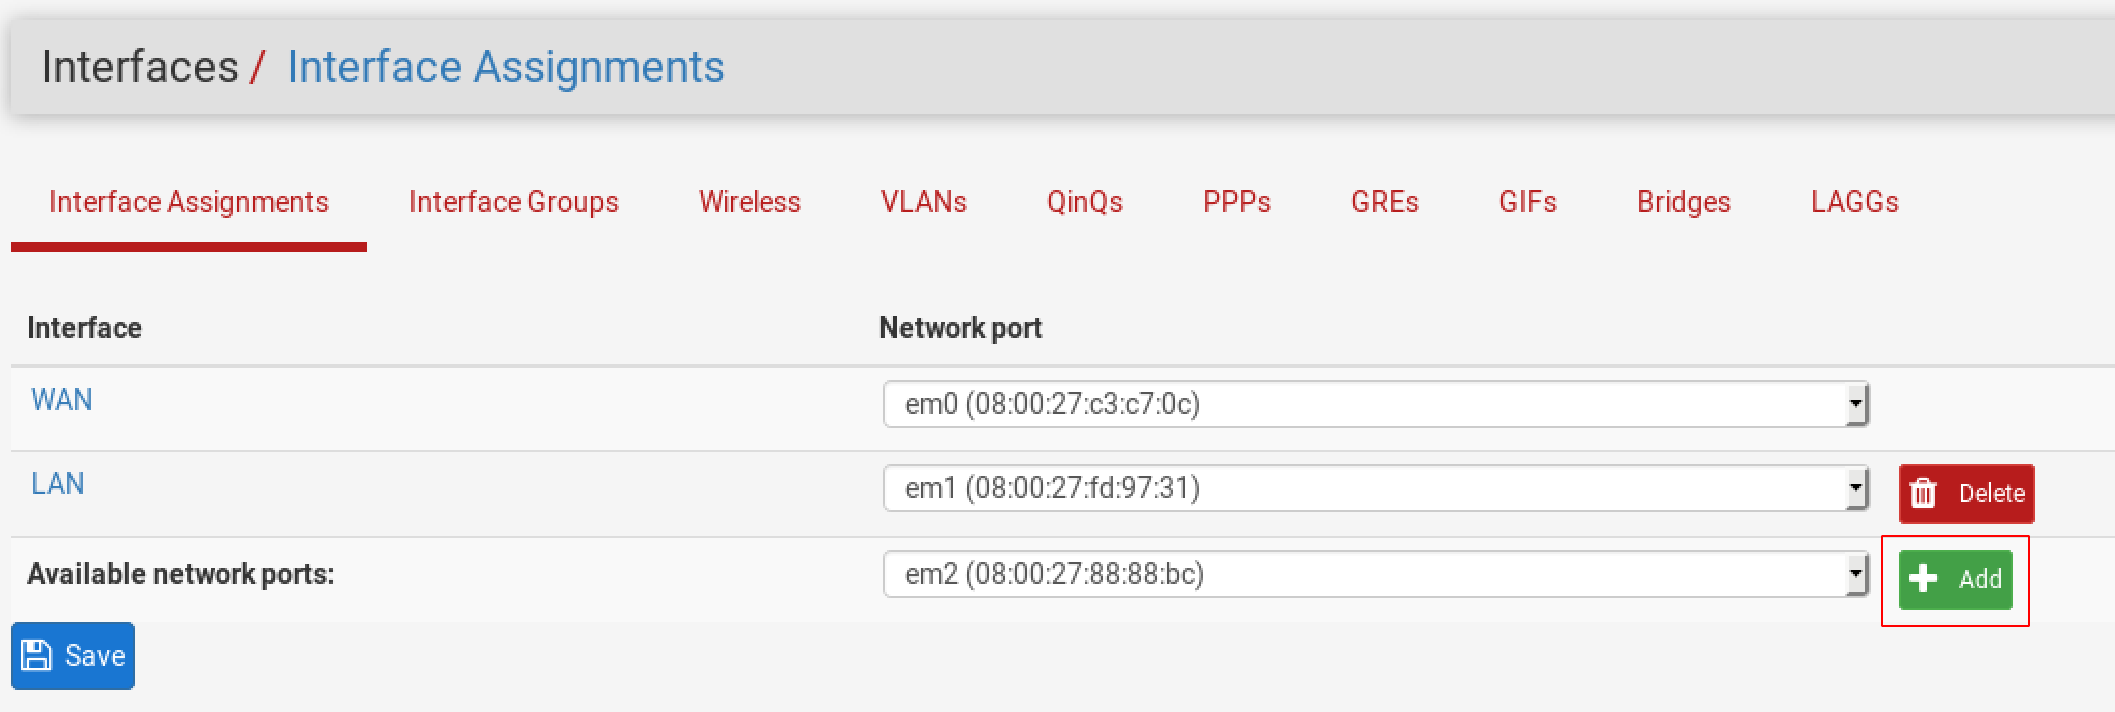
\includegraphics[scale=0.6]{Debian_screenshots/Config/9.png}
         \caption{Ajout d'une interface sur la page web de configuration de pfsense}
         \label{Debian_screenshots/Config/9}
     \end{center}
  \end{figure}
  \FloatBarrier
     
Cliquer sur la nouvelle interface créée, soit \textit{OPT1} :
  \begin{figure}[h!]
     \begin{center}
         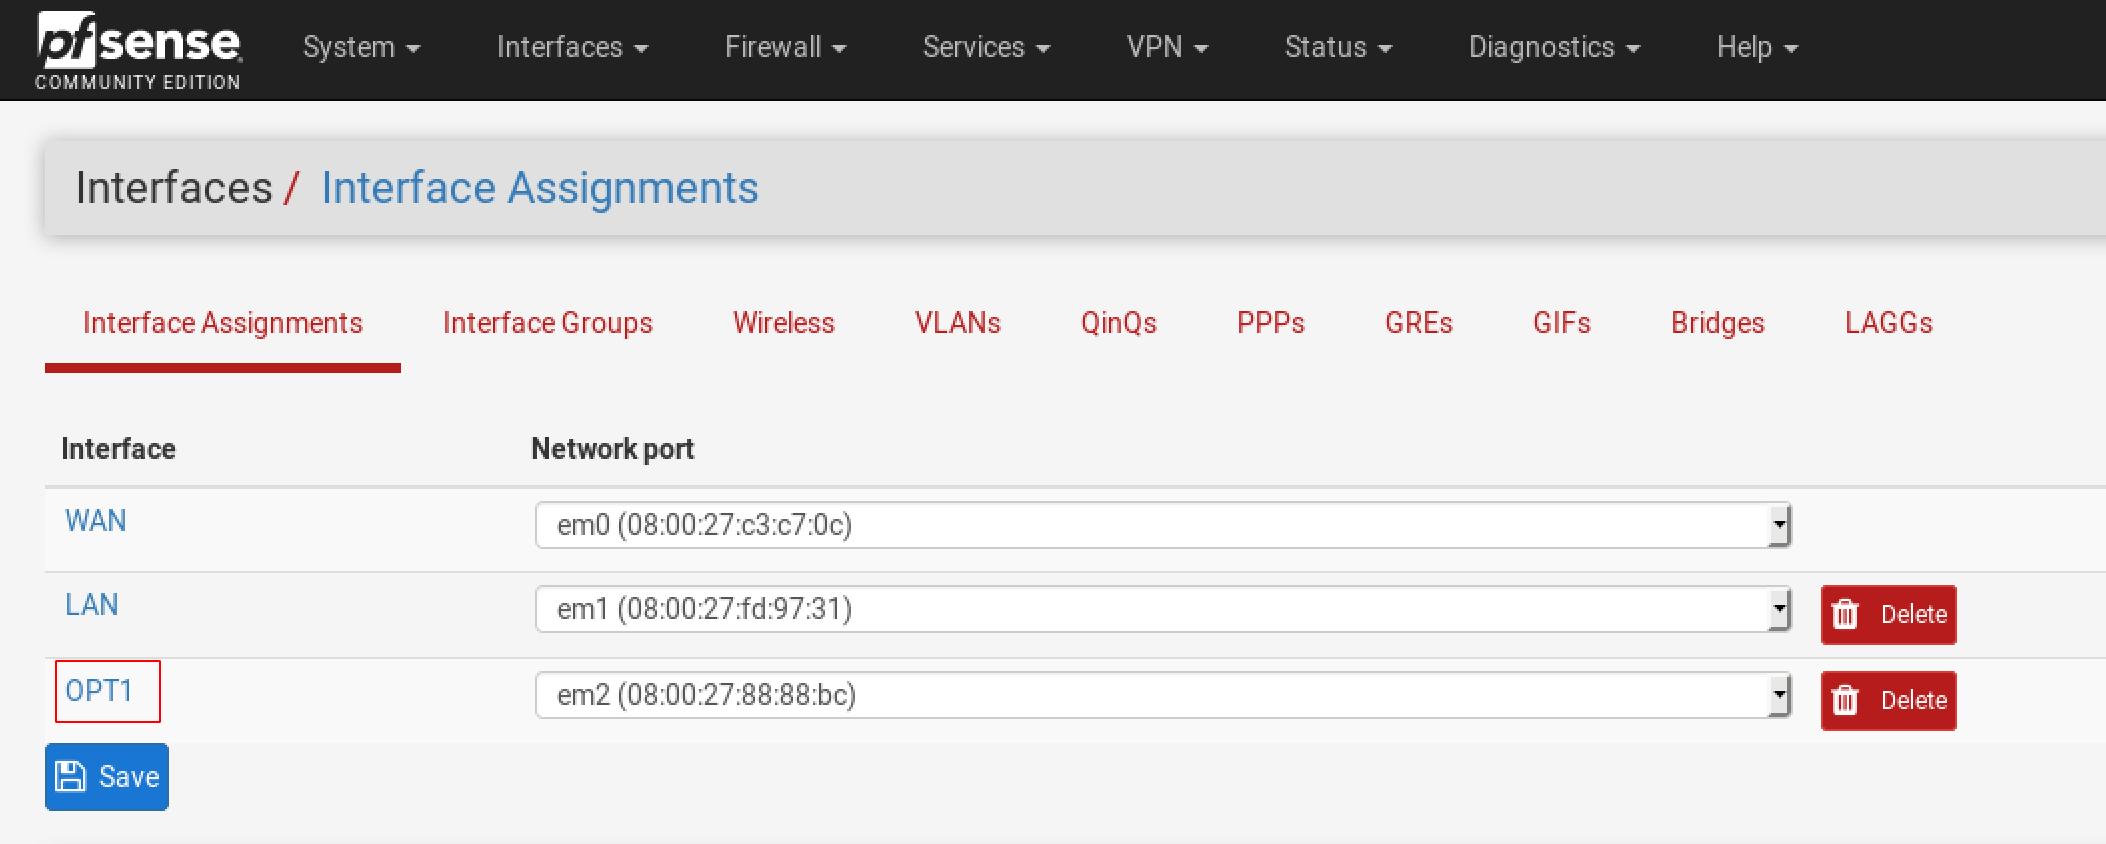
\includegraphics[scale=0.6]{Debian_screenshots/Config/10.png}
         \caption{Accès à la configuration de l'interface \textit{OPT1}}
         \label{Debian_screenshots/Config/10}
     \end{center}
  \end{figure}
  \FloatBarrier

\pagebreak
Remplir les champs comme sur la figure ci-dessous :
  \begin{figure}[h!]
     \begin{center}
         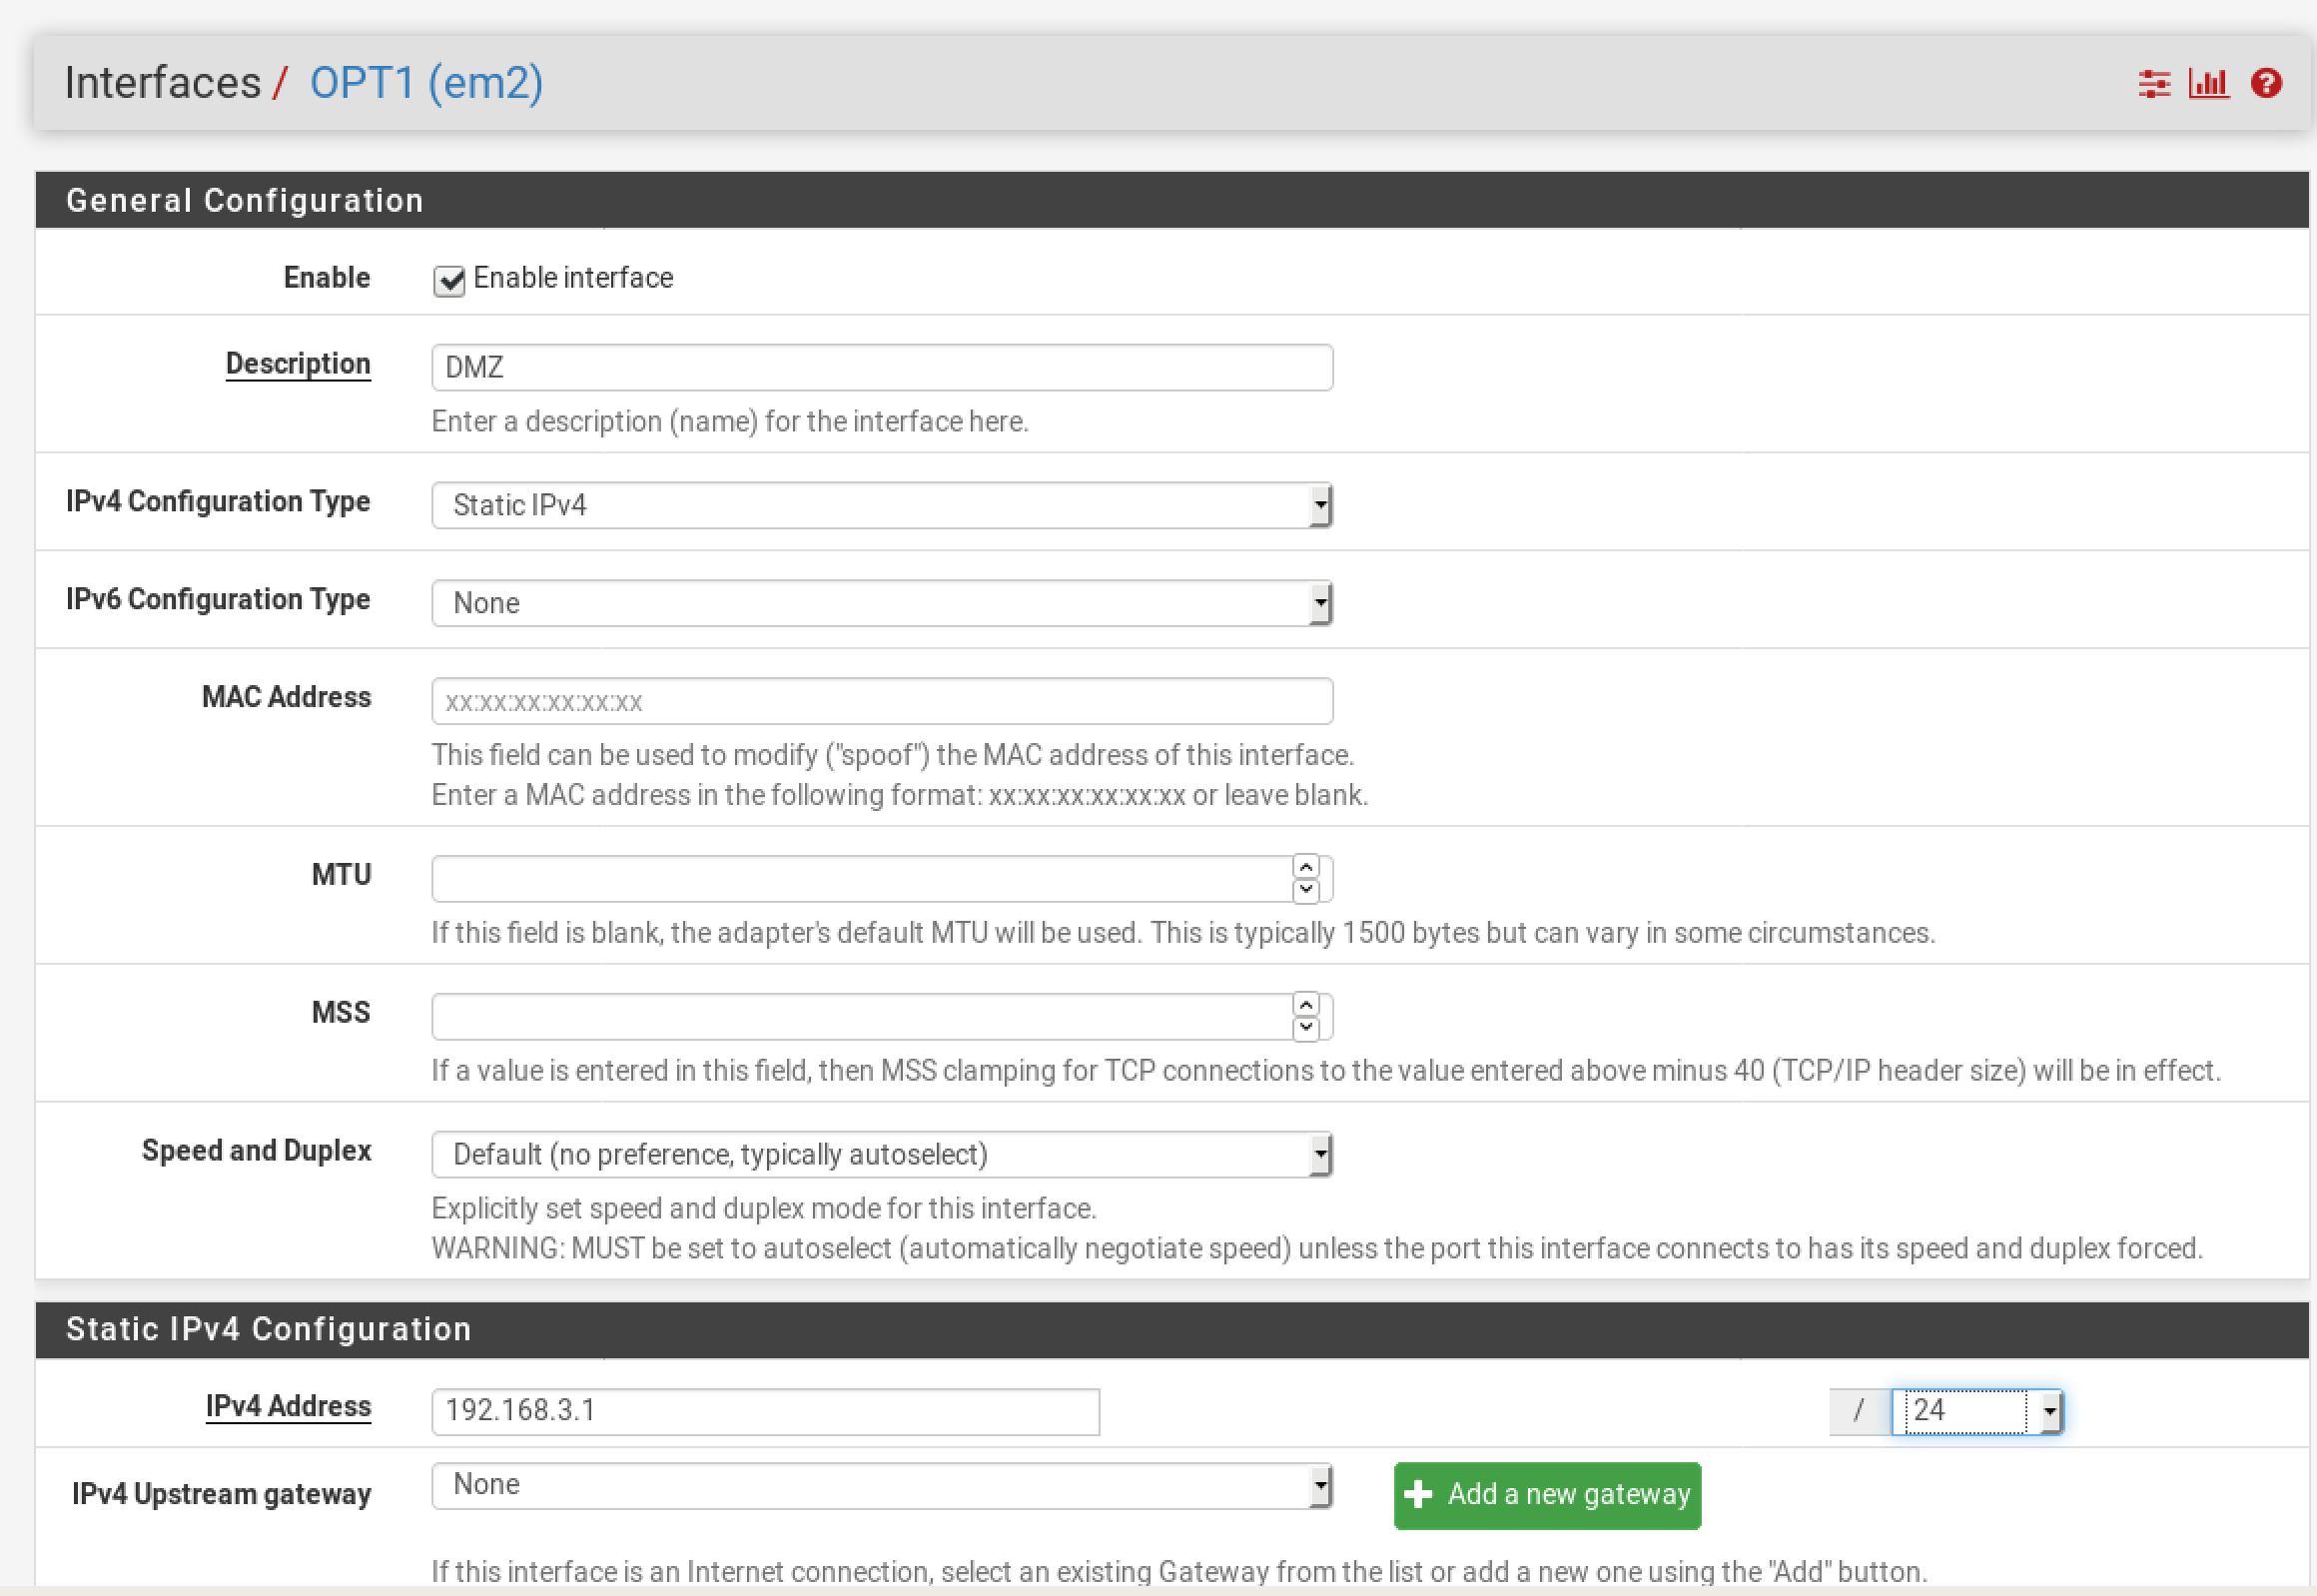
\includegraphics[scale=0.5]{Debian_screenshots/Config/11.png}
         \caption{Configuration de l'interface \textit{OPT1}}
         \label{Debian_screenshots/Config/11}
     \end{center}
  \end{figure}
  \FloatBarrier

\pagebreak
Cliquer sur le bouton \textit{Apply Changes} une fois les champs remplis :
  \begin{figure}[h!]
     \begin{center}
         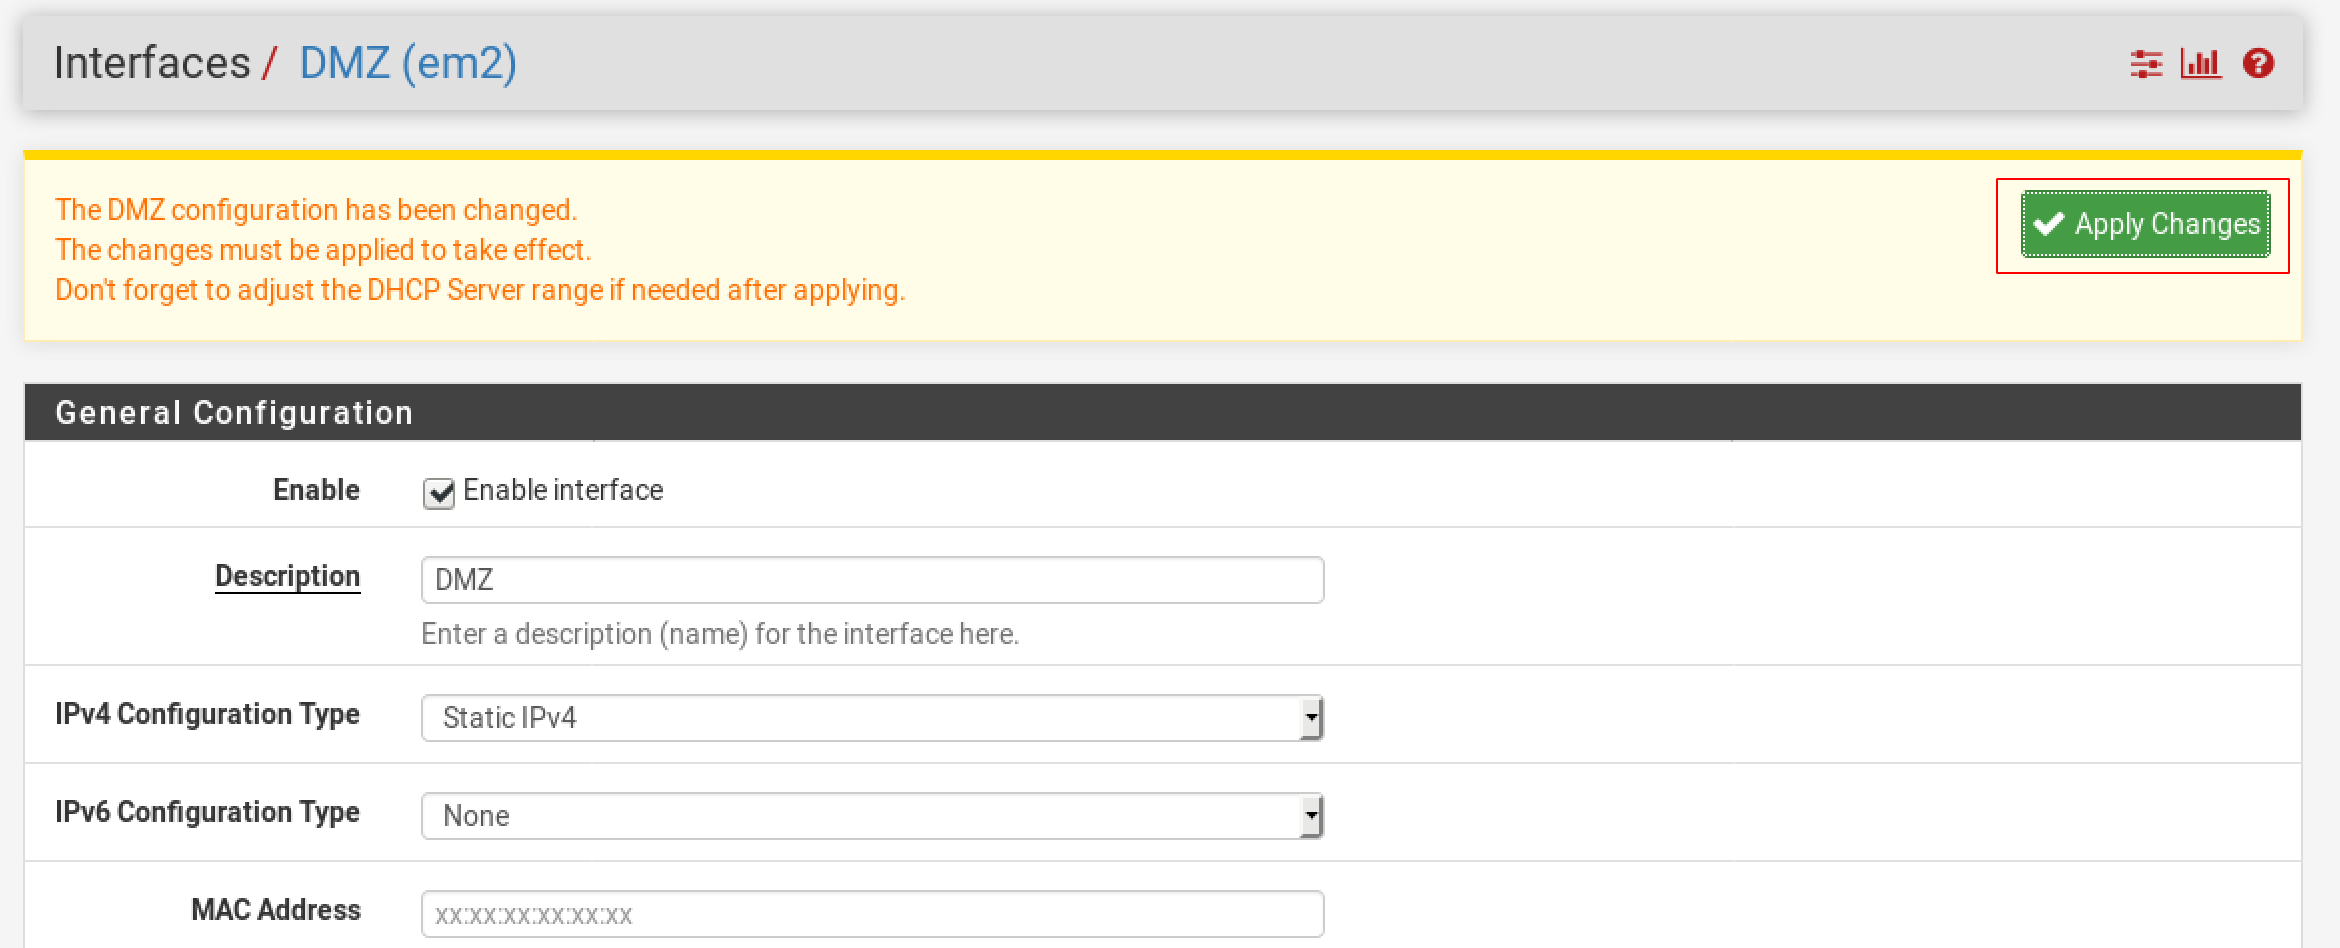
\includegraphics[scale=0.5]{Debian_screenshots/Config/12.png}
         \caption{Application des changements sur la configuration de l'interface}
         \label{Debian_screenshots/Config/12}
     \end{center}
  \end{figure}
  \FloatBarrier
     
Cliquer sur \textit{Firewall}, puis sur \textit{Rules} :
  \begin{figure}[h!]
     \begin{center}
         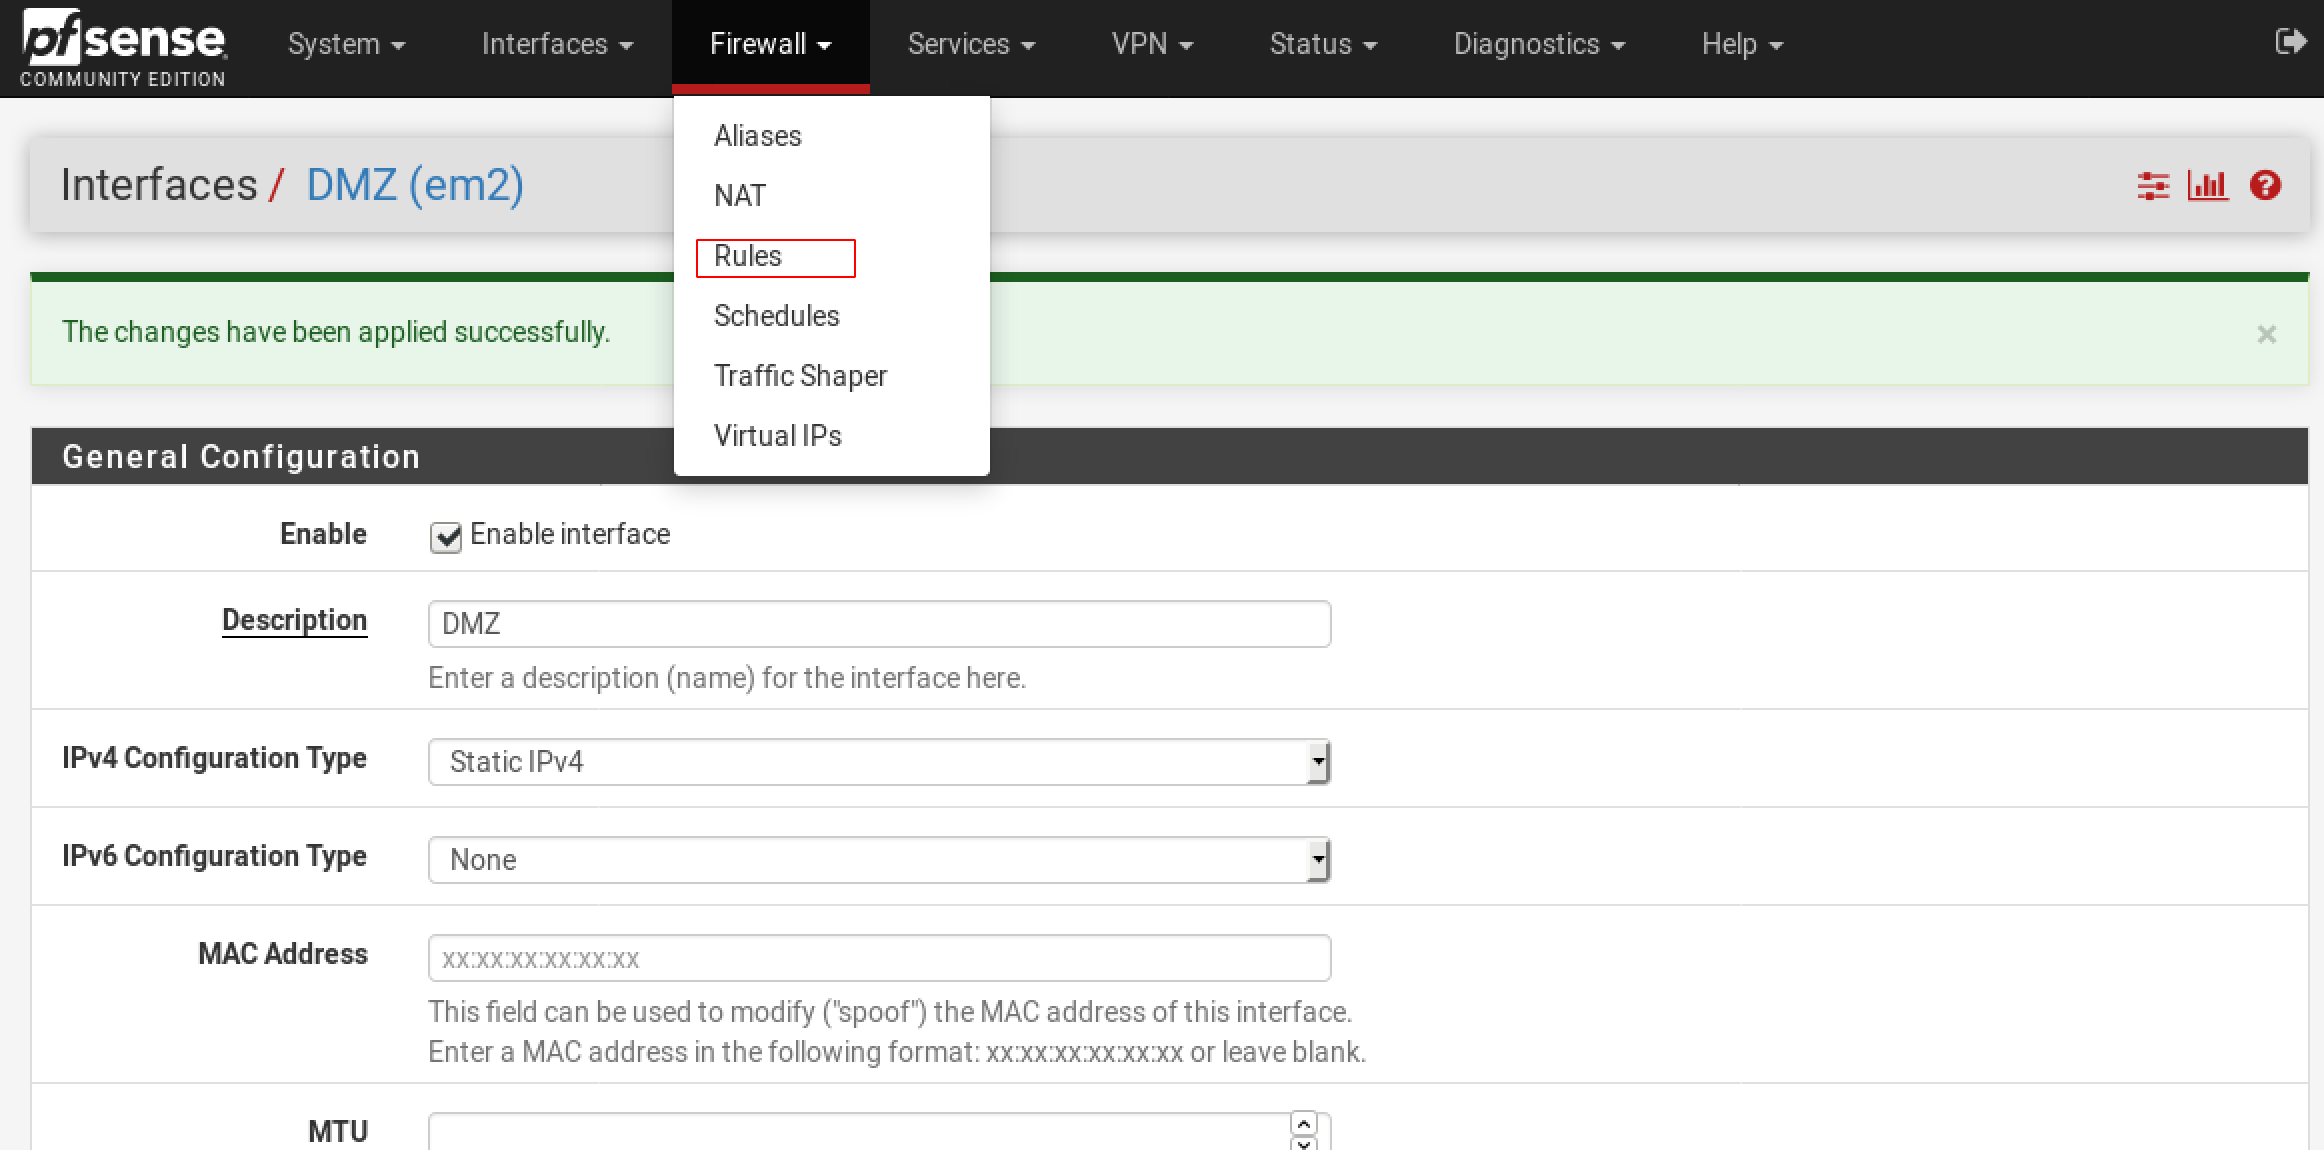
\includegraphics[scale=0.5]{Debian_screenshots/Config/13.png}
         \caption{Accès aux règles de pfsense sur l'interface web}
         \label{Debian_screenshots/Config/13}
     \end{center}
  \end{figure}
  \FloatBarrier

\pagebreak
Sélectionner la première règle ainsi que les deux dernières (d'après la figure suivante), puis cliquer sur le bouton \textit{Delete} :
  \begin{figure}[h!]
     \begin{center}
         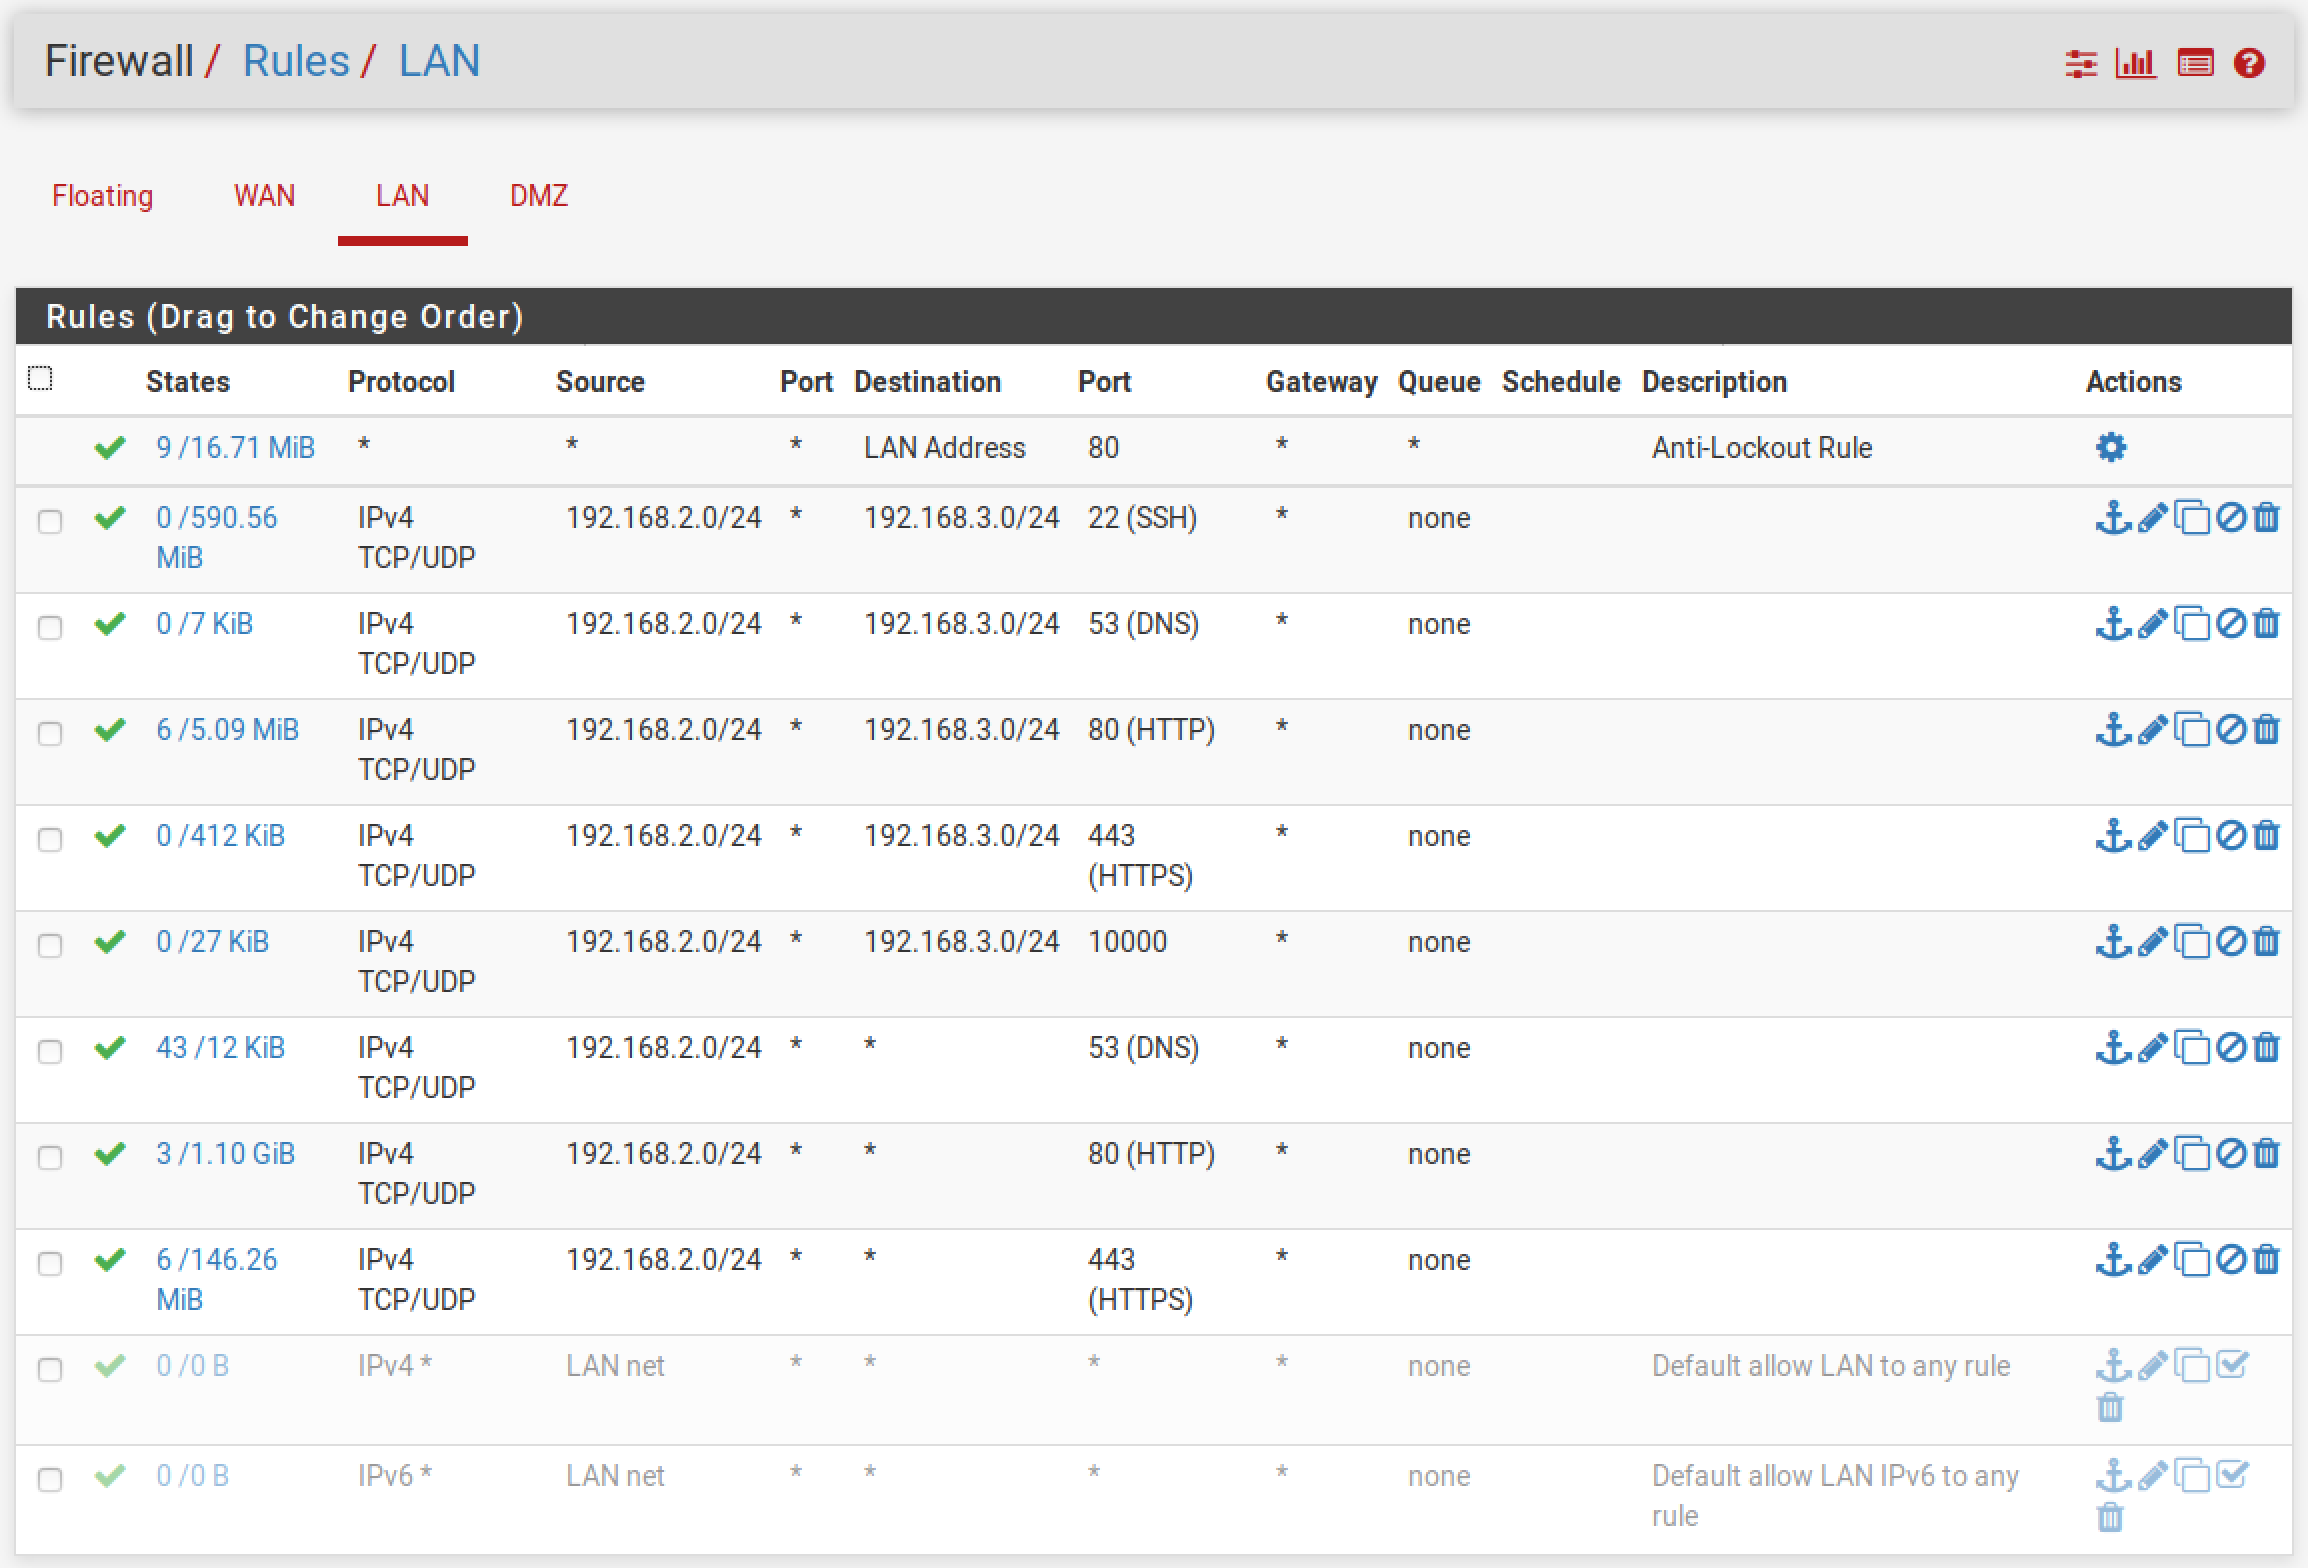
\includegraphics[scale=0.5]{Debian_screenshots/Config/14.png}
         \caption{Suppression de trois règles pfsense sur l'interface web}
         \label{Debian_screenshots/Config/14}
     \end{center}
  \end{figure}
  \FloatBarrier
     
Vérifier que la configuration des règles de pfsense soit la même que celle de la figure ci-dessous :
  \begin{figure}[h!]
     \begin{center}
         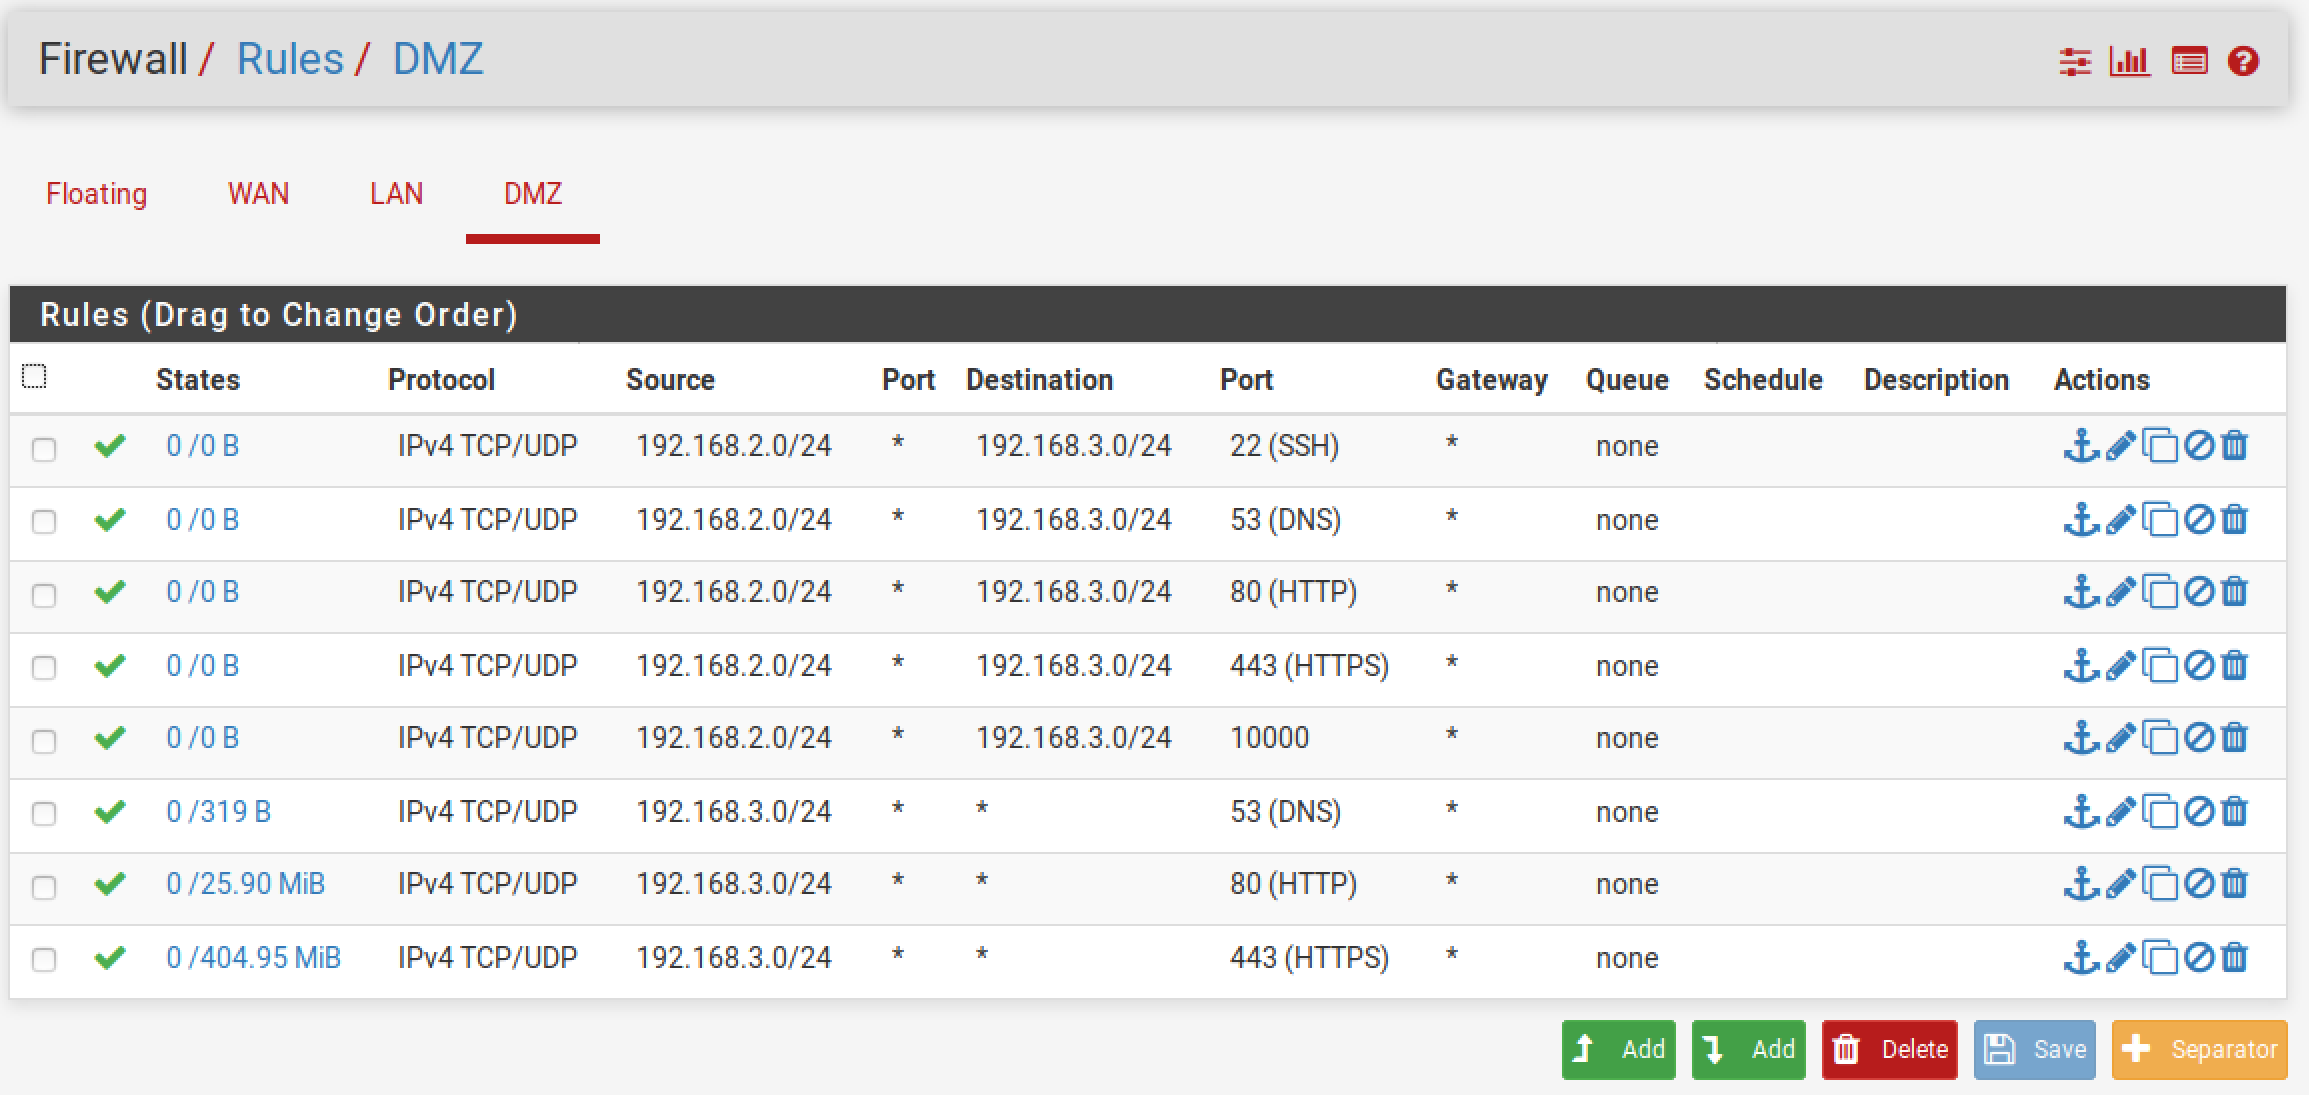
\includegraphics[scale=0.5]{Debian_screenshots/Config/15.png}
         \caption{Aperçu des règles de pfsense sur l'interface web}
         \label{Debian_screenshots/Config/15}
     \end{center}
  \end{figure}
  \FloatBarrier

\pagebreak
Cliquer sur l'icône pour les réseaux dans le coin haut-droite de la machine, puis cliquer sur \textit{Paramètres filaire} :
  \begin{figure}[h!]
     \begin{center}
         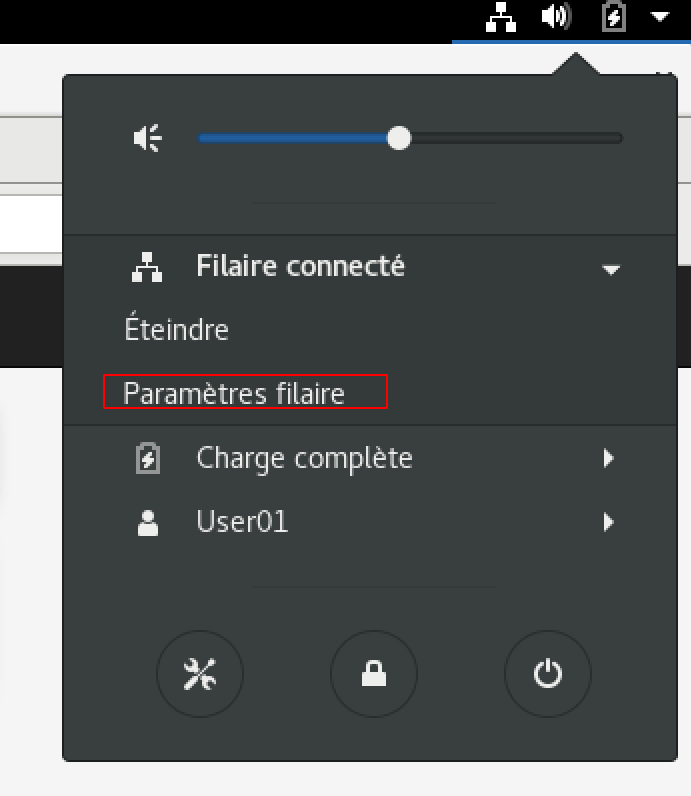
\includegraphics[scale=0.55]{Debian_screenshots/Config/16.png}
         \caption{Accéder aux paramètres filaire de la machine}
         \label{Debian_screenshots/Config/16}
     \end{center}
  \end{figure}
  \FloatBarrier

Aller dans la section \textit{IPv4}, puis sélectionner \textit{Manuel} afin de configurer les adresses suivantes : 192.168.3.2, 255.255.255.0 et 192.168.3.1. Cliquer sur \textit{Appliquer} :
  \begin{figure}[h!]
     \begin{center}
         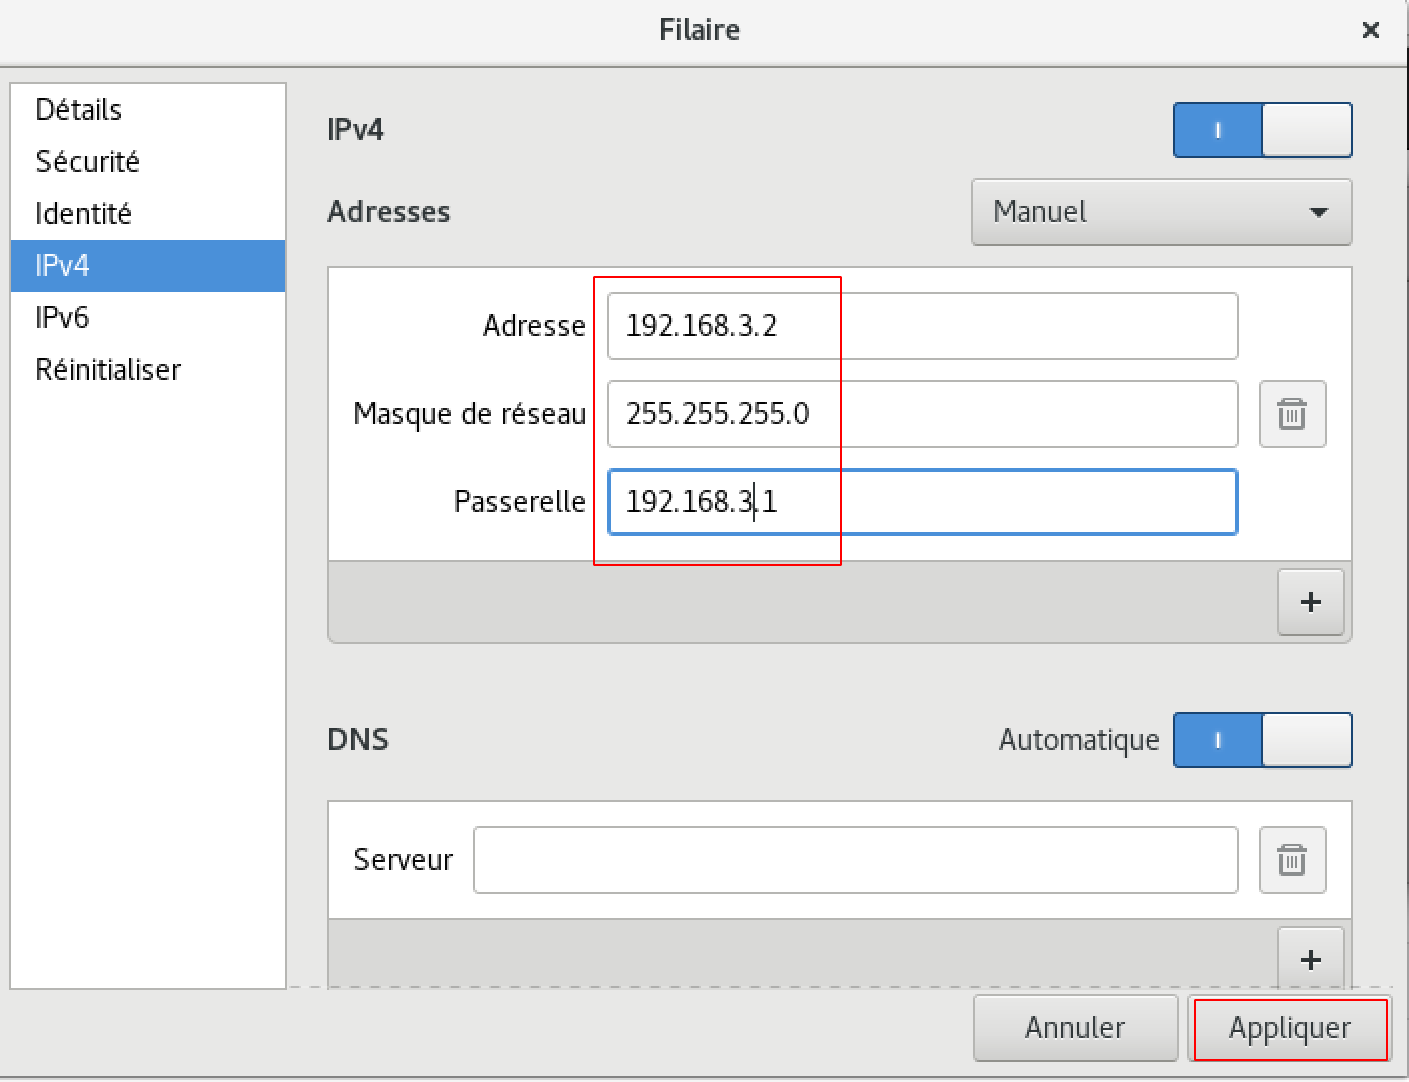
\includegraphics[scale=0.6]{Debian_screenshots/Config/17.png}
         \caption{Configuration des paramètres de connexion filaire en IPv4}
         \label{Debian_screenshots/Config/17}
     \end{center}
  \end{figure}
  \FloatBarrier

\pagebreak
Ouvrir la fenêtre de configuration réseau de la machine virtuelle Debian. Aller dans la section \textit{Réseau}, puis dans l'onglet "Interface 1", changer le nom à "dmz", puis cliquer sur \textit{OK} :
  \begin{figure}[h!]
     \begin{center}
         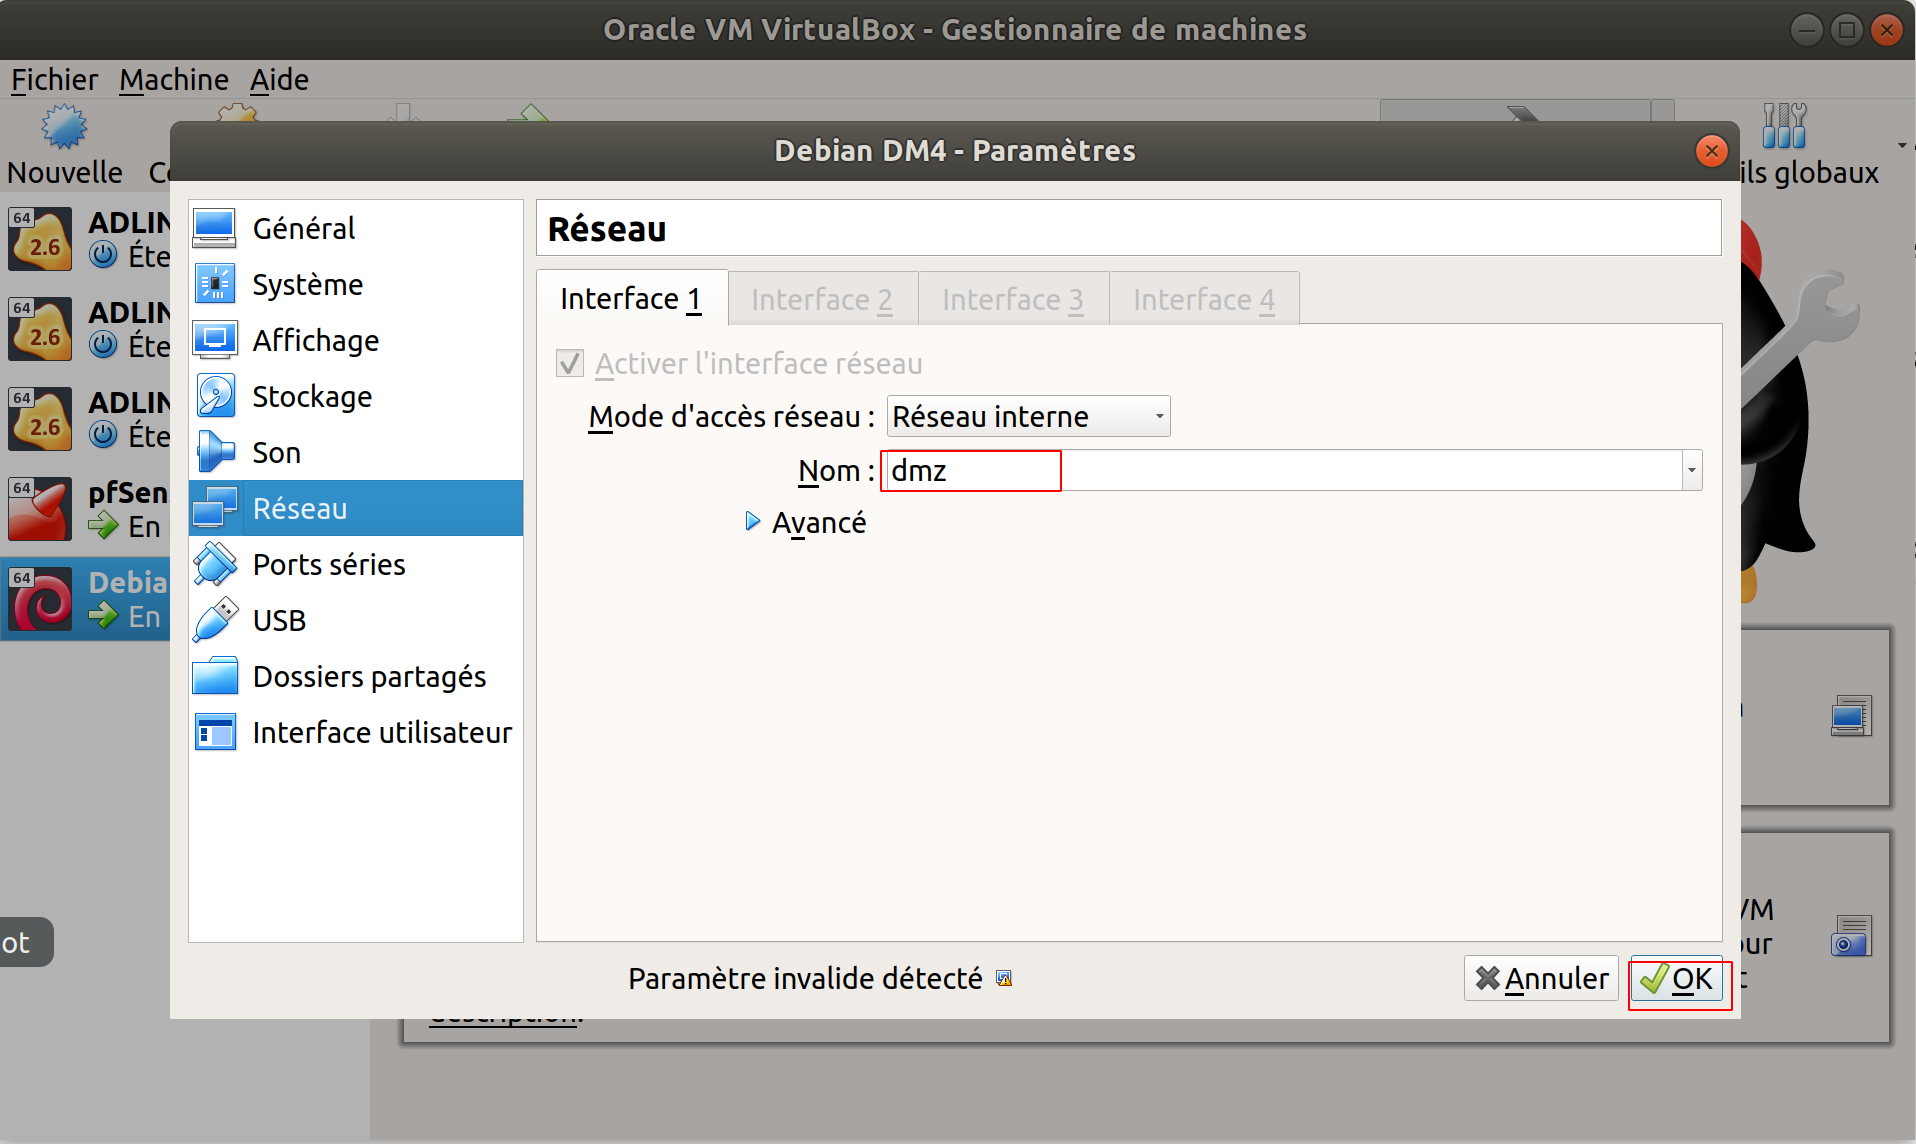
\includegraphics[scale=0.5]{Debian_screenshots/Config/18.png}
         \caption{Configuration réseau de la machine virtuelle Debian}
         \label{Debian_screenshots/Config/18}
     \end{center}
  \end{figure}
  \FloatBarrier
     
